%----------------------------------------------------------------------------------------
%                   Galway-Mayo Institute of Technology (GMIT)
%                Department of Computer Science and Applied Physics
%
%                      *** Latex template for dissertations ***
%----------------------------------------------------------------------------------------

\documentclass{report}

\usepackage{graphicx} % Required for the inclusion of images
\usepackage[numbers]{natbib} % Required to change bibliography style to APA
\usepackage{amsmath} % Required for some math elements 
\usepackage{makecell}
\usepackage{eurosym}
\usepackage{tabularx}
\usepackage{pbox}
\usepackage{listings}
\usepackage{xcolor}
\usepackage{url}
\setlength\parindent{0pt} % Removes all indentation from paragraphs


\definecolor{backcolour}{rgb}{0.95,0.95,0.92}
\definecolor{gray}{rgb}{0.4,0.4,0.4}
\definecolor{darkblue}{rgb}{0.0,0.0,0.6}
\definecolor{cyan}{rgb}{0.0,0.6,0.6}

\lstset{
  basicstyle=\ttfamily,
  columns=fullflexible,
  showstringspaces=false,
  commentstyle=\color{gray}\upshape
}

\lstdefinelanguage{XML}
{
  backgroundcolor=\color{backcolour},
  morestring=[b]",
  morestring=[s]{>}{<},
  morecomment=[s]{<?}{?>},
  stringstyle=\color{black},
  identifierstyle=\color{darkblue},
  keywordstyle=\color{cyan},
  morekeywords={xmlns,version,type}% list your attributes here
}

\lstdefinelanguage{JSON}
{
  backgroundcolor=\color{backcolour},
  morestring=[b]",
  morestring=[s]{"}{"},
  morecomment=[s]{<?}{?>},
  stringstyle=\color{black},
  identifierstyle=\color{darkblue},
  keywordstyle=\color{cyan},
}

\definecolor{maroon}{cmyk}{0, 0.87, 0.68, 0.32}
\definecolor{halfgray}{gray}{0.55}
\definecolor{ipython_frame}{RGB}{207, 207, 207}
\definecolor{ipython_bg}{RGB}{247, 247, 247}
\definecolor{ipython_red}{RGB}{186, 33, 33}
\definecolor{ipython_green}{RGB}{0, 128, 0}
\definecolor{ipython_cyan}{RGB}{64, 128, 128}
\definecolor{ipython_purple}{RGB}{170, 34, 255}
\definecolor{bluekeywords}{rgb}{0.13,0.13,1}
\definecolor{greencomments}{rgb}{0,0.5,0}
\definecolor{redstrings}{rgb}{0.9,0,0}

\lstset{
    breaklines=true,
    extendedchars=true,
    literate=
    {á}{{\'a}}1 {é}{{\'e}}1 {í}{{\'i}}1 {ó}{{\'o}}1 {ú}{{\'u}}1
    {Á}{{\'A}}1 {É}{{\'E}}1 {Í}{{\'I}}1 {Ó}{{\'O}}1 {Ú}{{\'U}}1
    {à}{{\`a}}1 {è}{{\`e}}1 {ì}{{\`i}}1 {ò}{{\`o}}1 {ù}{{\`u}}1
    {À}{{\`A}}1 {È}{{\'E}}1 {Ì}{{\`I}}1 {Ò}{{\`O}}1 {Ù}{{\`U}}1
    {ä}{{\"a}}1 {ë}{{\"e}}1 {ï}{{\"i}}1 {ö}{{\"o}}1 {ü}{{\"u}}1
    {Ä}{{\"A}}1 {Ë}{{\"E}}1 {Ï}{{\"I}}1 {Ö}{{\"O}}1 {Ü}{{\"U}}1
    {â}{{\^a}}1 {ê}{{\^e}}1 {î}{{\^i}}1 {ô}{{\^o}}1 {û}{{\^u}}1
    {Â}{{\^A}}1 {Ê}{{\^E}}1 {Î}{{\^I}}1 {Ô}{{\^O}}1 {Û}{{\^U}}1
    {œ}{{\oe}}1 {Œ}{{\OE}}1 {æ}{{\ae}}1 {Æ}{{\AE}}1 {ß}{{\ss}}1
    {ç}{{\c c}}1 {Ç}{{\c C}}1 {ø}{{\o}}1 {å}{{\r a}}1 {Å}{{\r A}}1
    {€}{{\EUR}}1 {£}{{\pounds}}1
}

\lstdefinelanguage{python}{
    morekeywords={access,and,break,class,continue,def,del,elif,else,except,exec,finally,for,from,global,if,import,in,is,lambda,not,or,pass,print,raise,return,try,while},
    morekeywords=[2]{abs,all,any,basestring,bin,bool,bytearray,callable,chr,classmethod,cmp,compile,complex,delattr,dict,dir,divmod,enumerate,eval,execfile,file,filter,float,format,frozenset,getattr,globals,hasattr,hash,help,hex,id,input,int,isinstance,issubclass,iter,len,list,locals,long,map,max,memoryview,min,next,object,oct,open,ord,pow,property,range,raw_input,reduce,reload,repr,reversed,round,set,setattr,slice,sorted,staticmethod,str,sum,super,tuple,type,unichr,unicode,vars,xrange,zip,apply,buffer,coerce,intern,string,public},
    sensitive=true,
    morecomment=[l]\#,
    morestring=[b]',
    morestring=[b]",
    morestring=[s]{'''}{'''},
    morestring=[s]{"""}{"""},
    morestring=[s]{r'}{'},
    morestring=[s]{r"}{"},
    morestring=[s]{r'''}{'''},
    morestring=[s]{r"""}{"""},
    morestring=[s]{u'}{'},
    morestring=[s]{u"}{"},
    morestring=[s]{u'''}{'''},
    morestring=[s]{u"""}{"""},
    % {replace}{replacement}{lenght of replace}
    % *{-}{-}{1} will not replace in comments and so on
    literate=
    {á}{{\'a}}1 {é}{{\'e}}1 {í}{{\'i}}1 {ó}{{\'o}}1 {ú}{{\'u}}1
    {Á}{{\'A}}1 {É}{{\'E}}1 {Í}{{\'I}}1 {Ó}{{\'O}}1 {Ú}{{\'U}}1
    {à}{{\`a}}1 {è}{{\`e}}1 {ì}{{\`i}}1 {ò}{{\`o}}1 {ù}{{\`u}}1
    {À}{{\`A}}1 {È}{{\'E}}1 {Ì}{{\`I}}1 {Ò}{{\`O}}1 {Ù}{{\`U}}1
    {ä}{{\"a}}1 {ë}{{\"e}}1 {ï}{{\"i}}1 {ö}{{\"o}}1 {ü}{{\"u}}1
    {Ä}{{\"A}}1 {Ë}{{\"E}}1 {Ï}{{\"I}}1 {Ö}{{\"O}}1 {Ü}{{\"U}}1
    {â}{{\^a}}1 {ê}{{\^e}}1 {î}{{\^i}}1 {ô}{{\^o}}1 {û}{{\^u}}1
    {Â}{{\^A}}1 {Ê}{{\^E}}1 {Î}{{\^I}}1 {Ô}{{\^O}}1 {Û}{{\^U}}1
    {œ}{{\oe}}1 {Œ}{{\OE}}1 {æ}{{\ae}}1 {Æ}{{\AE}}1 {ß}{{\ss}}1
    {ç}{{\c c}}1 {Ç}{{\c C}}1 {ø}{{\o}}1 {å}{{\r a}}1 {Å}{{\r A}}1
    {€}{{\EUR}}1 {£}{{\pounds}}1
    %
    {^}{{{\color{ipython_purple}\^{}}}}1
    {=}{{{\color{ipython_purple}=}}}1
    %
    {+}{{{\color{ipython_purple}+}}}1
    {*}{{{\color{ipython_purple}$^\ast$}}}1
    {/}{{{\color{ipython_purple}/}}}1
    %
    {+=}{{{+=}}}1
    {-=}{{{-=}}}1
    {*=}{{{$^\ast$=}}}1
    {/=}{{{/=}}}1,
    literate=
    *{-}{{{\color{ipython_purple}-}}}1
     {?}{{{\color{ipython_purple}?}}}1,
    %
    identifierstyle=\color{black}\ttfamily,
    commentstyle=\color{ipython_cyan}\ttfamily,
    stringstyle=\color{ipython_red}\ttfamily,
    keepspaces=true,
    showspaces=false,
    showstringspaces=false,
    rulecolor=\color{ipython_frame},
    frame=single,
    frameround={t}{t}{t}{t},
    framexleftmargin=6mm,
    numbers=left,
    numberstyle=\tiny\color{halfgray},
    backgroundcolor=\color{ipython_bg},
    % extendedchars=true,
    basicstyle=\scriptsize,
    keywordstyle=\color{ipython_green}\ttfamily,
}

\lstdefinelanguage{csharp}{
  showspaces=false,
  showtabs=false,
  breaklines=true,
  showstringspaces=false,
  breakatwhitespace=true,
  escapeinside={(*@}{@*)},
  commentstyle=\color{greencomments},
  keywordstyle=\color{bluekeywords},
  stringstyle=\color{redstrings},
  basicstyle=\ttfamily
}

\newcommand*{\customTitle}{\begingroup % Create the command for including the title page in the document
\centering % Center all text
\vspace*{\baselineskip} % White space at the top of the page

\rule{\textwidth}{1.6pt}\vspace*{-\baselineskip}\vspace*{2pt} % Thick horizontal line
\rule{\textwidth}{0.4pt}\\[\baselineskip] % Thin horizontal line

%----------------------------------------------------------------------------------------
%	1) Change Dissertation Title
%----------------------------------------------------------------------------------------
{\Large VIRTUAL REALITY CONFLICT RESOLUTION APPLICATION}\\[0.2\baselineskip] % Title
%----------------------------------------------------------------------------------------


\rule{\textwidth}{0.4pt}\vspace*{-\baselineskip}\vspace{3.2pt} % Thin horizontal line
\rule{\textwidth}{1.6pt}\\[\baselineskip] % Thick horizontal line
\scshape % Small caps \\[\baselineskip] % Tagline(s) or further description
\Large \textbf{Final Year Project}\\
\textbf{B.Sc.(Hons) in Software Development}\par % Location and year
\normalsize
\vspace*{2\baselineskip} % Whitespace between location/year and editors


%----------------------------------------------------------------------------------------
%	2) Change Student Name(s)
%----------------------------------------------------------------------------------------
{\textbf{By} \\ Aaron Hannon \\ Matthew Sloyan \par} % Editor list
%----------------------------------------------------------------------------------------

\medskip

{\textbf{GitHub Link:} \\ https://github.com/MatthewSloyan/final-year-applied-project-and-minor-dissertation \par}

\vspace*{2\baselineskip} % Whitespace between location/year and editors
\vfill % Whitespace between editor names and publisher logo
{\scshape \today} \\[0.3\baselineskip] % Year published
%----------------------------------------------------------------------------------------


%----------------------------------------------------------------------------------------
%	3) Change Supervisor
%----------------------------------------------------------------------------------------

{\textbf{Advised by Damien Costello}}\par % Supervisor

{Department of Computer Science and Applied Physics Galway-Mayo Institute of Technology (GMIT)}\par % Department
%----------------------------------------------------------------------------------------


\endgroup}
\begin{document} 
\pagenumbering{gobble}
\begin{figure}
\begin{center}

\includegraphics[width=8cm,height=3.3cm,keepaspectratio]{gmit-logo} % Include the image placeholder.png
\end{center}
\end{figure}
\customTitle % This command includes the title page
\tableofcontents
\listoffigures
\pagenumbering{arabic} 



%----------------------------------------------------------------------------------------
%	4) Change Chapters
%      Write each chapter in a separate TEX file and include here
%----------------------------------------------------------------------------------------

\chapter{Introduction}

\section{Application Description}
This application is a virtual reality training simulation for ICSE security . The function of the application is to reduce training costs while training ticket inspectors on the Luas in Dublin. Currently they have to hire actors and close off a Luas route to train new inspectors and this project helps eliminate that. Once you launch the application on the virtual reality headset you are in a virtual train station. As soon as you hop on a train it disembarks then commencing the training session. The goal is to check everyone's ticket on board the train by conversing with all the non-player characters (NPCs) using your actual voice and they will reply to you using a text-to-speech engine. All the NPCs have different personalities so this is where the conflict resolution aspect of the project comes in. You may come across someone who maybe very rude and you must coerce them into giving you their ticket or you may be fortunate to talk to someone who gives you their ticket straight away. Once all the NPCs are checked you may leave the train, check your score and end the simulation. After the purchase of a virtual reality headset there is very little cost involve and the training simulation can be replayed over and over again completely removing the need to hire actors and shutdown a Luas route for an entire day.  

\section{Client}
Mark Toner who works for ICSE security, contacted our supervisor to propose a project. The project entailed creating a training simulation for ticket inspectors for the Luas in Dublin. The Problem with their current training system is that they have to hire out a large number of actors to act like passengers. Also they have to close off one of the Luas's routes to ensure the setting for the training session is as accurate as possible. The problem with this method was it is extremely costly to recreate this every time new people need training as they would have to hire actors again and close of a Luas route. So we were tasked with creating an application that was as useful in training ticket inspectors to deal with conflict resolution as it was cost effective. After meeting with Mark we came up with some application ideas. In the end we settled on a virtual reality training simulation that allowed you to speak to bots, they would interpret what you are saying and respond. Also these bots had to have different personalities or personas. The simulation had to have variance with each bot so to not make it too easy for the trainee. Some bots could be nice and some could be extremely rude. After this meeting we started research and development straight away.

\section{Objectives}
Here are the main objectives that were decided after having a meeting with our client.

\begin{itemize}
    \item To make sure that we, as developers, understood the requirements of the client to help us develop a system that the client was content with. 
    
    \item To research the latest technology to aid in creating an application that would not be out-dated and that it was as efficient as possible for the time.
    
    \item To Implement a robust system architecture what we have learnt from our research of the latest technologies.
    
    \item To create an application that we, as developers, were happy with but more importantly, creating a product that met the requirements of our client.
    
\end{itemize}

\section{Scope}
This project was from the start treated as industry standard so we knew that the scope was large however, manageable and we knew that we could meet all the requirements in the time frame that was given to us. During the course of the project we had to set up:
\begin{itemize}
    \item Create a virtual realistic environment for the training session to take place with life-like models and animations
    
    \item Speech services that would convert speech to text then text to speech in a realistic fashion.
    
    \item Create chat-bots that would recognise what you were saying with the aid of an artificial intelligence.
    \item Create a back-end server where the 3D engine/client could communicate with the chat-bot.
    
    \item Set-up a hosting service for the server so 3D engine/client did not have to be on the same network to function.
    
\end{itemize}

Although there was a lot here to research and implement we were confident that we would get the project done in the given time frame.


\section{Chapter Overviews}
Here is a brief overview of the all the following chapters. These chapters include Methodologies, Technology Review, System Design, System Evaluation and the conclusion to the entire project.
\subsection{Methodologies}
In chapter 2 we discuss all the various methodologies we used throughout the research and development of the project. We also mention how we interacted with our client and project supervisor. There is also a big emphasis on testing, management and the tools used to aid us in development. 
\subsection{Technology Review}
In chapter 3 we outline all the technologies we either used in development or that we researched and tested however did not suite our requirements. To summarise what kind of technologies we research, we looked at 3D Engines/ Gaming Engines, Speech services that would allow us to convert Speech to text and vice versa, relevant chat-bot technologies, various servers that we could use to aid us in developing an efficient back-end to process HTTP requests and finally hosting services for our back-end server. 
\subsection{System Design}
In chapter 4 we examine the entire implementation of the application in detail. We go through all the technologies that met our requirements from the Technology Review and what roll they played in creating our project. Code snippets are also used to aid our explanation of the implementation and to show the inner workings for each section in the application.
\subsection{System Evaluation}
In chapter 5 we mainly focus on the actual performance and robustness of the system which are described in the Objectives section of this chapter. We answer questions like how well does the system perform when tested. We also look at any technical limitations that we encountered during the projects life-cycle. 
\subsection{Conclusion}
In the final chapter we conclude this document as a whole. We highlight any findings from the system evaluations section. We also look at objectives and see how well we met them.

\section{Source Code}
The entirety of the this project can be located on GitHub. Upon clicking the link below you should be able to see the project's repository containing all source code and documentation related to the project. The "Chatbot" folder contains the AIML bot's source that was used in the project and a sample bot using the Keras machine learning library. The "Research" folder contains a "Initial Research.md" file that contains all the research that was completed before starting the development stage. The "UnityEngine" folder contains the entire Unity project including all scripts and assets. Finally, there is a "README.md" file that shows all information regarding trying to run the project.
\newline

GitHub Link: https://github.com/MatthewSloyan/final-year-applied-project-and-minor-dissertation

\section{Deliverables}
Listed below are all the components to be included in the project derived from the clients requirements:

\begin{itemize}
    \item A Virtual reality application with a 3D train station environment and realistic non-player characters that you can converse with, developed using Unity3D that is to be launched on the Oculus Quest.
    
    \item A live Flask server hosted on PythonAnywhere so that the Unity3D can connect and access the chat bot to generate replies and return it to the user to give the illusion of a conversation.
    
    \item A Mongo database that contains all the data of previous training sessions so that the trainees progress or score can be reviewed to see how well they deal with conflict resolution. 
\end{itemize}
\newpage
\section{Workload Breakdown}
In this section we will break down all the work we individually did that made it into the final build throughout the projects life's life cycle. Below is the list of the list of the work done (Not necessarily in chronological order)

\subsection{Aaron Hannon's Work}
\begin{itemize}
    \item AIML bot implementation.
    \item Flask server with AIML implementation and hosted on PythonAnywhere.
    \item Created Unity3D environment With non-playable characters(NPCs).
    \item NPCs have genders and different personas.
    \item Created a client script that allowed Unity to communicate to.
    \item Added character controller allowing the user to navigate through the scene for testing when not built to the Oculus.
\end{itemize}


\subsection{Matthew Sloyan's Work}
\begin{itemize}
    \item Implemented Azure speech services allowing us to convert speech to text and text to speech.
    \item Oculus Support added and implemented allowing the user to navigate the scene using the Oculus Quest.
    \item Added various voices types to the NPCs.
    \item Menus that function with the Oculus and implemented Oculus controls.
    \item The scoring system and pushing data to a Mongo database.
    \item Added game/simulation over screen.
\end{itemize}

\chapter{Methodology}
This chapter will look at the methodologies we used throughout the project regarding research, software development, client \& supervisor meetings, testing, project management and the tools used.

\section{Research Methodology}
For this project we chose a form of a Mixed Research Methodology which involves both Qualitative and Quantitative research. 

\subsection{Qualitative}
Qualitative research is focused on exploring and finding out thoughts, ideas and opinions. This was suitable for our project at an early stage such as meeting the client initially. From this we gained invaluable insights into his goals, thoughts and ideas for the prototype. We also were given possible scenarios for the training application. An example was a ticket inspector (The player) would board the train and would be able to interact with any passenger to check if they had a ticket. From this scenario we conducted research into multiple areas such as chatbot technology, gamification and much more. 

\subsection{Quantitative}
Quantitative research is less theoretical than qualitative research and is focused more on numerical results and statistics. This research was used later in development when we had developed and deployed a test build. These builds were shown the client and our supervisor. In return we collected the feedback, thoughts and ideas they had which was used to further make changes and achieve the initial outlined goals.

\section{Software Development Methodology}
We looked at several different approaches regarding software development methodologies, which included Waterfall and Agile methodologies. Waterfall is a sequential series steps or processes that must be completed before moving onto the following steps. These processes include (Requirements, Design, Implementation, Verification and Maintenance). However, from initial research we decided it wouldn't suit our projects as it can exclude the client from the process, cause changes to be difficult to make and delay testing till the end of the project which would decrease software quality. Another methodology we looked at was Agile. Agile promotes continuous development, deployment and testing throughout the software development life cycle (SDLC) of the project to help increase productivity, software quality and decrease development time. We felt this would be most suitable to our project so we began to look at how Agile could be implemented to coincide with our initial goals.

\subsection{Agile - Extreme Programming}
The Agile methodology we have chosen for this project was Extreme Programming (XP). Extreme Programming is a form of Agile, which focuses on small development teams, quick iterative development cycles and a focus on test driven development. It is based on five values simplicity, communication, feedback, courage and respect. \cite[p.~4]{1335275620040101}. 

\begin{figure}[h!]
	\caption{Extreme Programming Life Cycle.}
	\label{image:XP}
	\centering
	
\includegraphics[width=0.65\textwidth]{Images/Extreme_Programming.png}
\end{figure}	

\subsubsection{Advantages}
\begin{itemize}
  \item Cuts down cost and time of software projects, due to a focus on timely delivery of final products and less time on cumbersome documentation. Also, problems are solved through group discussions and errors are spotted earlier with Peer reviews. Peer reviews involve two programmers sitting side by side working on a feature. This was helpful for us working in college as we could fix bugs quickly and efficiently.
  \item Feedback is constant, so changes can be made quickly and efficiently.
  \item Software is developed faster, due to constant testing and deployment.
  \item Simplicity is key, so code can be developed quickly to pass tests and meet goals, and then improved later.
  \item Works well with small and large teams.
\end{itemize}

\subsubsection{Disadvantages}
\begin{itemize}
  \item Not suitable for teams that separated geographically.
  \item There can be a lack of defect documentation, so bugs can go unnoticed or not tested. However, we improved on this with GitHub issue tracking.
  \item The lack of full documentation can cause problems especially in larger projects or if team members leave/join midway.
\end{itemize}

As the advantages outweigh the disadvantages it was clear XP was the correct methodology to choose. Also, since it is more suited to the team size, workflow, project type and client.

\section{Meetings}
Initially we met with both our supervisor and our client. In this meeting we discussed initial goals, thoughts and ideas for the project (Qualitative Research). We also outlined the minimum requirements for the prototype which are described in the introduction chapter. Each week we would then meet our supervisor to discuss the following.

\begin{itemize}
  \item Our progress from the last meeting.
  \item Feedback on our progress.
  \item Our next steps and planning.
  \item Answer any questions from our client or supervisor. 
\end{itemize}

The frequency of meetings fitted well with XP perfectly as we could make any changes that arose from the meeting, then test and deploy the project again for the following week to show our supervisor.

\section{Testing}
Throughout the project we incorporated multiple testing methodologies such as Functional and Non-functional testing. More information on how these methodologies were implemented can found in the System Evaluation chapter.

\subsection{Functional Testing}
Functional testing focuses the functional aspects of a system such as unit, integration and system testing.

\subsubsection{Unit testing}
Unit testing is the first form of testing to be completed and is usually undertaken by the developer themselves. It involves testing a class level, E.g. testing functions in a class if they behave correctly and don't produce errors. We implemented tests using NUnit framework to test basic functions of the Unity game. We also used pytest to run unit tests on the server, and to test the HTTP methods from the application to the server we used Postman to check the packets and debug errors.

\subsubsection{Integration testing}
Integration testing involves testing the system to insure it still works when adding new features, so it doesn't break other areas of the system. We implemented integration by testing for all aspects of the system to see if they still worked correctly on all iterative builds. This was especially useful when adding Oculus VR support as it caused errors with the speech services.

\subsubsection{System testing}
System testing is a black box testing methodology completed after integration testing to ensure the system meets the requirements. We implemented system testing by ensuring the application met the initial requirements outlined by the client in the Introduction Chapter.

\subsection{Non-functional Testing}
Non-functional testing focuses the non-functional aspects of a system such as performance, usability and compatibility.

\subsubsection{Performance testing}
Compatibility testing is a measure of how the system performs under pressure, or heavy load. We tested the system with a high number of requests to the server to ensure it didn't buckle under load.

\subsubsection{Security testing}
Security testing involves testing how secure the system against unauthorized attack. We implemented security measures regarding the server, deployment and database access.

\subsubsection{Usability testing}
Usability testing involves measuring the ease of use from and end user’s perspective. This was vital to our game as it's a training experience, so we spent a lot of time working on improving usability of all controls, menus and game play. We conducted user tests with multiple users and our supervisor to collect data.

\subsubsection{Compatibility testing}
Compatibility testing is a measure of how well a system works in different environments (Browsers, devices etc.). This was essential as we were developing the application to work on Android, Windows, and Oculus Quest VR.

\section{Project Management}
We have used Git with GitHub to track our changes, log error and work effectively using our chosen Agile methodology. Git is an open source and free version control system which allows small or large projects to be stored and accessed efficiently. Features include commits, branching, staging and workflows. It can be connected to GitHub which allows a project to be stored remotely and for multiple people to work together seamlessly. 

\par
\medskip

Using GitHub and Git allowed us to work simultaneously on the project to increase our productivity. We also used the inbuilt features on GitHub such as issue tracking. If an issue occurred or a bug was found during testing, we would make a GitHub issue, and log all our commits using the issue id. This would track our progress in fixing it and help us keep an account of the work undertaken.

\section{Development Tools}
For this project we used a multitude of tools to develop each section. The main tool that was used was the Unity Editor and Visual Studio. The Unity version used was 2019.2.6f1 which includes all the new features and provided support for the Azure Speech Services used. All the Unity script were written using Visual Studio in C\#. Visual Studio was useful as it included the required packages and IntelliSense for creating Unity scripts. The flask server was developed using Visual Studio code and was initially deployed to an AWS EC2 (Amazon Elastic Computer Cloud). Later it was deployed and modified using Heroku, and then finally PythonAnywhere.

\chapter{Technology Review}
\section{Overview}
This chapter looks at some of the technologies used throughout the project with a focus on why we choose them along with the benefits they possess. Also, covered is some of the technology researched and reviewed which was not used but lead us to our final implementation. The technologies include:

\begin{itemize}
    \item What 3D Engine to use?
    \item What Speech Service?
    \item What technology to create a chat-bot?
    \item What Back-end?
\end{itemize}

\section{Application}
We knew knew we would need some form of gaming engine for the application itself. This would be the part for the project that the user would actually interact with. There are number of free gaming engines that we could have used however, we chose the Unity Engine as it is very well documented and powerful enough for our needs.

\subsection{Unity}
This is the part of the application is where the user interacts with. After briefly looking at other game engines we chose unity it for below reasons:

\begin{itemize}
  \item Unity uses C\#. The reason this is good is because C\# is very versatile and supports many different programming styles. It can be used to created objects, make network requests and it is also Unity's default scripting language.
  \item It was apparent that 3D models and animations would be key to improving the experience of the application. Unity allowed us to add 3D models ease. Unity also has a built in animator that allows you to animate these models by key-framing them and moving them as desired. All of this was very important to create a realistic training experience for the user.
  \item Another aspect that was important was to be able to connect to our back-end Flask server. Unity has built in HTTP support allowing us to send necessary JSON data from the Speech-to-Text service to the server to be processed and a response sent back.
  \item As mentioned Speech-to-Text (STT) and Text-to-Speech (TTS) is another important feature that was needed to enhance the realism for the user. After some research we found out that a lot the STT and TTS services support Unity and supply their own packages for the engine, giving us options for when we decided on which STT and TTS service we were going to choose.
\end{itemize}

% Packages for STT & TTS

\section{HTTP}
HTTP or HyperText Transfer Protocol is a protocol used by the world wide web to send messages to from a client to a server or vice verse. It also defines how these messages are structured to inform the server or web browser what actions to take upon receiving a request. The reason we chose this approach is because for one Unity has libraries that handle incoming and outgoing HTTP requests. Also it Flask uses HTTP making it very easy to communicate with our back-end server.

\section{Virtual Reality (VR)}
\subsection{Google VR}
Lit Review..
\subsection{Oculus Quest}
Lit Review..

\section{Speech Services}
As the application needed to include a dynamic chatbot we looked as some areas such Text-to-Speech (TTS) and Speech-to-Text (STT) services to achieve this. Our initial thought was to include a text input system or a multiple choice dialog tree but from testing and further research we felt it would be pre-programmed and substantially less interactive for a training environment. This spurred us to look at other areas and the possibility of taking in audio from the microphone and parsing it to text using TTS. TTS involves converting human speech to a text format so it can be read by a machine in real time. On the other hand, STT is the opposite in which text is converted to human like synthesized speech, which would be used to give our chatbot life, personality and evoke possible emotions. Below we will look at some of the technologies we reviewed and tested in these two areas.

\subsection{Windows}
All Windows devices have STT functionality built into its Cortana virtual assistant. This allows the user to talk directly to the device and it will pick up what you said and decide from this. As described above we decided to use Unity as the main technology for our application which would be deployed to and Oculus Quest, so any service we tested must work with Unity and Android respectively. As the Windows STT services provided a Unity package, we thought it could work well, however from testing it was quite slow at depicting speech despite being accurate. Also, the text predicted was lower case and contained no punctuation, or any useful characters such as question marks etc. which would be useful for determining context in Natural Language processing. Another unfortunate downside was that it didn't work on Android when testing so we decided to look at other options, this was since it's developed for Windows. 

\subsection{Google Cloud}
The second speech service we looked at was Google Cloud Speech Synthesis. Compared to the inbuilt system provided by Windows this service works using an application programming interface (API) where audio data is sent to a remote server and a result is returned. Because of this a constant internet connection is required which is another issue to look at. Using the documentation provided a solution was implemented despite it not working as desired due to the fact there is no specific Unity package available. The only way to implement it to implement the DLL files in Unity as a source which worked but unfortunately not as desired. Another area where Google Cloud was quite beneficial was the fact that allowed the developer to tailor the Speech Services to their own need. Some options included the ability to change the voice of the response from TTS or changing the pitch and tone of the voice. This would be useful for depicting emotion in characters. The cost to use Google's services was also quite reasonable and provided a good allowance of free usage which would suffice for our needs but as it didn't work as expected we decided to test other services. 

\subsection{IBM Watson}
Another service we researched was IBM Watson speech services, but with only a very limited amount of free characters (10,000) available for TTS and 250 minutes free with STT we found it to be a costly service to use. Another downside again to this service was the fact that there was no Unity package available either, so ultimately, we decided to look into other service providers.

\subsection{Azure}
Much like Google Cloud services Azure works in much the same way and provides the same features regarding multiple voices, tone, pitch etc. which would allow a realistic experience. There is also over 140 different voices provided with 9 specific Neural voices built using machine learning that are specifically designed to provide a realistic human like response. Also, there is support for over 45 languages which could be used for future research to make the application available in multiple countries. Other benefits include the fact there is a Unity package available for both TTS and STT, along with Android, IOS and Windows support. Another feature which improves on the inbuilt Windows STT is the service can depict punctuation and other useful characters such as question marks etc. which would be useful for Natural Language processing (NLP). Below we will look a more in-dept look at the costs for each service in relation to virtual training.

\subsubsection{Costs - Azure Text-to-Speech}
There would be 250-400 replies an hour on average, with around 12500-20000 characters used per hour (average sentence around 50 characters). Based on the above the free tier would allow up to 25 hours of training for free per month. Additional characters can be purchased for 14 EUR (1 million characters) which would allow for an additional 50 hours of training.

\subsubsection{Costs - Azure Speech-to-Speech}
Every reply is on average 3-10 seconds. In one hour of training, it will use around 30 minutes. Based on the above the free tier would allow for up to 10 hours of training for free per month (5 hours free). A further hour can be purchased for 0.80 EUR, which equates to 2 hours of training. So, an additional 10 hours of training would cost 4.00 EUR.
\newline\newline
From testing, research and analysis of the benefits we decided to use Microsoft Azure services for our application for the following reasons.

\begin{itemize}
  \item Azure provided the best training cost, which would be useful for our client.
  \item Azure provided the most useful custom options in regard to multiple voices, language, pitch tone etc. which would required to scale the project in the future.
  \item Azure STT works extremely well at depicting human speech and includes punctuation. It is also very efficient and accurate.
  \item A Unity package is provided which would allow it to be easily deployed to a Unity environment and run efficiently.
  \item Android and IOS are supported which would allow the service to work on the multiple VR devices reviewed such as the Oculus Quest and Google VR.
\end{itemize}

\section{Chatbot}
It was a given that a we needed to create a chat-bot so this was one of the first areas we started to research. We looked at all the chat-bots created in the past and they all followed a trend. This trend was that they either used machine learning or AIML also known as Artificial Intelligence Markup Language. Before deciding on one from the beginning we tested both technologies to see which was suited best to our requirements. All we needed the bot to do at the start was take in an input and return an accurate and relevant response. Before implementing Speech-to-Text and Text-to-Speech we worked with the most simple for of conveying dialog which was strings of text. We got this working with both the AIML and machine learning
approach. Below are the two technologies in more detail and why when chose AIML.

\subsection{Keras}
Keras is a deep learning library that allows you to create neural networks quickly with very little implementation. It also has a dedicated library for python which would run seamlessly on our flask server meaning we could make requests to the neural network using HTTP. To train the model, we processed a JSON intents file that included objects that looked like this:

\begin{lstlisting}[language=JSON]
{"intents": [
    {"tag": "greeting",
     "patterns": ["Hi.", "Is anyone there?", "Hello.", "Good day"
        , "Whats up?"],
     "responses": ["Hello!", "Good to see you again!", "Hi there
        , how can I help?"],
     "context_set": ""
    },
    {"tag": "greetingResponse",
      "patterns": ["I am great thanks!", "Great, thank you!"
        , "Not too bad!"],
      "responses": ["That's good to hear.", "I'm glad."],
      "context_set": ""
     }
    ]
}
\end{lstlisting}

The pre-processing mapped certain words to the tag. For example in the above snippet you can see the tag "greeting", and one of the patterns is "Is anyone there?". What the pre-processing does is it creates a bag for words related to the tag removing any unnecessary words like "Is" in the case. Then it trains the model using this tag and that bag of words. It also has a list of responses that added to the output of the neural network. After training the model keras loaded it and it was ready for use. Pre-processing would have to be done for every input to. This was done using the the method of creating a bag for words. Then that bag of words was used as an input to predict an output/response. The neural network was very accurate however it had some issues:

\begin{itemize}
  \item The model would have to be rebuilt every time more responses where appended to the intents file making it tedious and bulky to maintain.
  \item There was no simple way for creating independent sessions for each bot. This was a feature that we really needed as we knew the application would have many different instances of the bot and that progress/state needed to be saved and there was no simple way of doing it.
\end{itemize}

Initially the we thought the safest approach in creating a chat-bot would be to use a neural network however, after doing some testing and a working build using keras we found out that it was not the right route to take.

\subsection{AIML}
%https://www.tutorialspoint.com/aiml/aiml_tutorial.pdf
Artificial Intelligence Markup Language (AIML) is markup language that allows you to create a set of conversation rules. These rules contain various tags and symbols that allow you to generate outputs or responses based on the input. AIML's tags are similar to another markup language called Extensible Markup Language(XML). The reason these markup languages are so similar is due to the fact that AIML is derived from XML. The main reason we chose AIML over the Keras approach was for the simple reason that we needed to store session data. This would have been very difficult to do using keras and would have forced us to do a lot of string manipulation to try and extract the relevant data from the input. AIML had built in tags and methods that allowed us to save various bits of data that we could store on a session by session basis. This was essential to the project and that is why we fundamentally chose AIML over Keras.
\newline

Below is a table of the tags that are most used in AIML and a description of what they do:
\newline
\begin{tabular}{ |p{3cm}|p{10cm}|  }
\hline
\multicolumn{2}{|c|}{AIML TAGS} \\
\hline
Tag & Description \\
\hline
$<$ aiml $>$ & Defines the beginning and end of a AIML document. \\
\hline
$<$ category $>$ & Defines the unit of knowledge in a bot's knowledge base. \\
\hline
$<$ pattern $>$ & Defines the pattern to match what a user may input to a bot. \\
\hline
$<$ template $>$ & Defines the response of a bot to user's input. \\
\hline
$<$ star $>$ & Used to match wild card * character(s) in the $<$pattern$>$ Tag. \\
\hline
$<$ srai $>$ & Multipurpose tag, used to call/match the other categories. \\
\hline
$<$ random $>$ & Used $<$random$>$to get random responses. \\
\hline
$<$ li $>$ & Used to represent multiple responses. \\
\hline
$<$ set $>$ & Used to set value in an AIML variable. \\
\hline
$<$ get $>$ & Used to get value stored in an AIML variable. \\
\hline
$<$ that $>$ & Used in AIML to respond based on the context. \\
\hline
$<$ topic $>$ & Used in AIML to store a context so that later conversation can be done based on
that context. \\
\hline
$<$ think $>$ & Used in AIML to store a variable without notifying the user. \\
\hline
$<$ condition $>$ & Similar to switch statements in programming language. It helps the bot to respond
to matching input.\\
\hline
\end{tabular}
\newline
\newline

Below is a snippet of the simplest input and output that can be made in AIML. When the user says "HELLO BOT" AIML looks for patterns that contain this string. If the pattern is found, the bot replies with the contents of the template tags which is "Hello User!". However, if the input is not found in the patterns, you can have a catagory that acts as a catch all using the "*" symbol which will become the default response if no other input was found which in this case would be "Sorry, I do not understand...".

\begin{lstlisting}[language=XML]
<aiml version="1.0.1" encoding="UTF-8"?>
    <category>
    <pattern> HELLO BOT </pattern>
        <template>
            Hello User!
        </template>
    </category>
    
    <category>
    <pattern> * </pattern>
        <template>
            Sorry, I do not understand...
        </template>
    </category>
</aiml>

\end{lstlisting}

With the AIML file set up all we had to do was access it through our flask server. We were fortunate that python has an AIML library that handles reading the file and saving the state for the chat-bots. Saving the states of every bot was essential for this project that is why we picked AIML.



\section{Back-end}
\subsection{Node}

\subsection{Flask}
Flask is a web framework that allows you to build web applications with ease. Flask is actually classed as micro-framework meaning it has very little dependencies to external library. This means Flask is extremely light-weight therefore, very efficient. Because we were working with STT and TTS efficiency was key. We needed to be able to generate responses as quickly as possible to give the illusion that you were having an actual in person conversation with the bot. Flask had this capability along with it being simple to set up so that is why we used it to host the back-end of this application. Below is a snippet of python code to set up a simple working server:

\begin{lstlisting}[language=PYTHON]
from flask import Flask
app = Flask(__name__)

@app.route("/")
def hello():
    return "Hello World!"

if __name__ == "__main__":
    app.run()

\end{lstlisting}

\section{Back-end - Deployment}
After developing and deciding on using Flask as our back-end, we needed to host the server and deploy it in a production build so it could be accessible to devices outside of the local network. A debug server for testing in Flask can only take one request at a time so it's not scalable or secure, so a production build is required. Below is a list of the different options for deploying a Flask server.

\subsection{Self-hosted Options}
Self-hosted solution can be deployed using Web Server Gateway Interface (WSGI) containers. This specification is used to describe how a web service communicates with web applications. A few examples of WSGI containers include Gunicorn, uWSGI, Gevent and Twisted Web. We attempted to implement a WSGI on a Windows Amazon Web Service (AWS) virtual machine (VM) but from research these types of servers are best suited to Linux machines, so we decided to look into other options.

\subsection{Hosted Options - Cloud Services}
There is various platform as a service (PaaS) solutions available to deploy a production server to, which we will look at below. PasS is a model provided by third party vendors, where the vendor hosts the hardware and software on their own virtual machines and provides access at an affordable cost, which is usually much cheaper than setting up your own machines. Below we will review two options that we assessed, tested and used for development.

\subsubsection{Heroku}
Heroku is a PasS which allows developers to build, run and deploy applications easily and efficiently to the cloud. Git version control software is used to update, modify and deploy quickly. Heroku also provides a free tier services for student so it is a cost-effective approach to allowing applications to be easily accessible around the world, which is what we required to access our server from an Oculus Quest VR device. There was a few downsides to Heroku though. The first one being an issue with AIML. AIML allows you to store session data/variables which would enable you to save names and other data relevant to each NPC. Heroku had a problem storing this session data making it very difficult to save the states if all the different NPCs/bots in the application so we had to find a different deployment service. Another issue we found was that Heroku would timeout quickly if there was no incoming requests. This made the initial request slow to respond because you would have to wait for Heroku to launch the server.

\subsubsection{PythonAnywhere}
PythonAnywhere is what we decided to use after testing Heroku. It is very similar to Heroku as it allow developers to build, run and deploy their applications on the cloud. However, it differs in a few ways. The free tier of PythonAnywhere allowed the server to stay live for 3 months at a time making initial requests to the flask server much quicker. You could also opt for a paid tier which keeps it live based on a certain amount of usage but the free tier was perfect for testing. Another way that it differs from Heroku is that there is no Git version control instead using an online IDE on their site which allows you to edit all your files from anywhere on any device. Finally the main reason we choose PythonAnywhere, it did not have the issue with saved AIML sessions that Heroku did. This was a deal breaker for us because we needed these sessions for the bots and without them it would have been very difficult to save the states for the bots. 

\section{Databases}
\subsection{MongoDB}

\section{Other areas of research}
As outlined in our introduction the focus of this application was to provide a realistic and gamified training experience that would be useful to the user specifically in the area of conflict resolution. To succeed with this we researched areas such as Digital Twins, Sara de Freitas, Michael J Sutton, Serious Fun, Gamification and Digital Training/VR Training.
\chapter{System Design}

\section{Overview}
In this section, we will illustrate the entire system in detail. We will go through all the various technologies that were finalized from the technical review, where they are located in the project structure and what role they have in creating a fluid and realistic experience for the user. In Figure~\ref{image:SystemArch} we can see the high-level design of the project and how all the technologies we have developed connect. Each component has a major role to play in creating this fluid experience and we will discuss how they were implemented in detail.

\begin{figure}[h!]
	\caption{System Architecture.}
	\label{image:SystemArch}
	\centering
	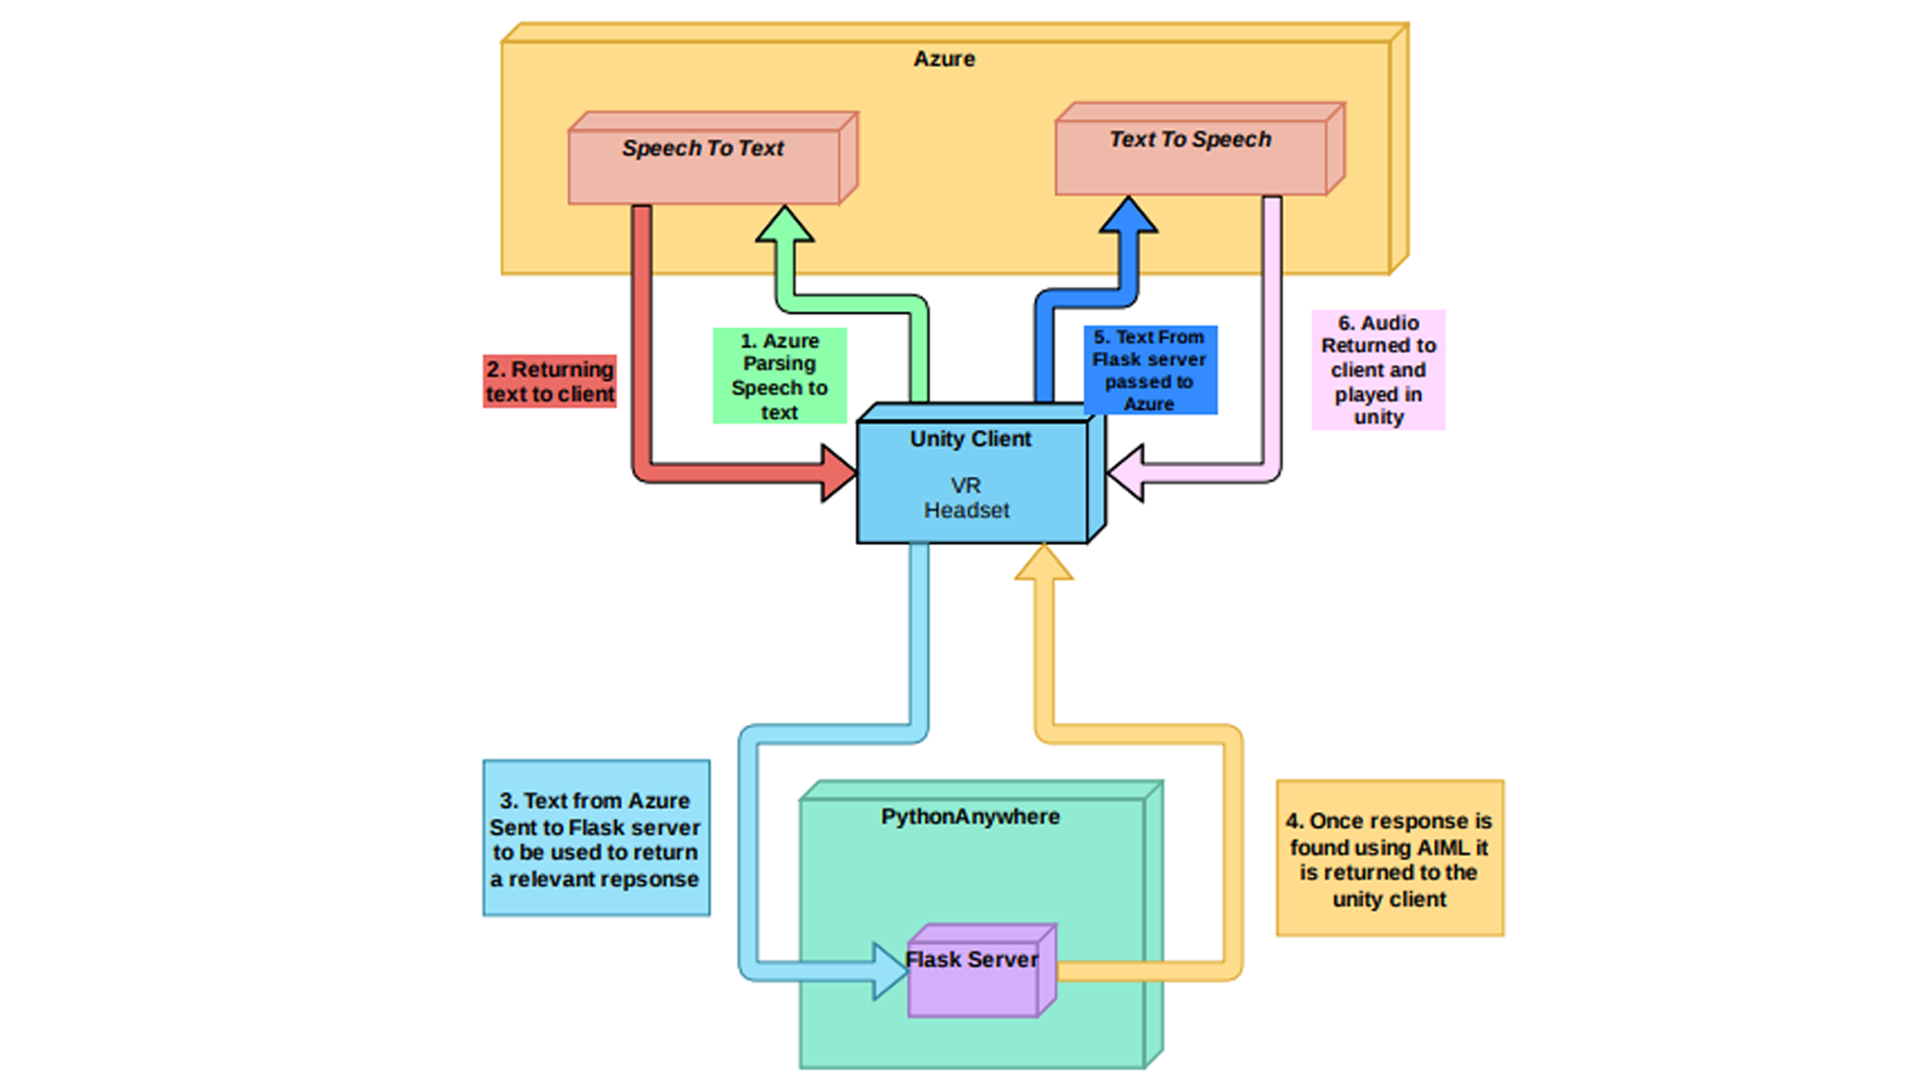
\includegraphics[width=1\textwidth]{Images/uml2.png}
\end{figure}

\section{Unity}
As seen in figure~\ref{image:SystemArch} Unity is the central component to this application. It is the part that the user interacts with and the part where all the data flows in and out of. Figure~\ref{image:ClassDiagram} describes the whole Unity system at a class level. In this section and whole chapter we will look at this class diagram in more detail and describe how some of the features work. We will also explore the graphical side of the implementation and how we achieved that.

\begin{figure}[h!]
	\caption{Unity Project Class Diagram.}
	\label{image:ClassDiagram}
	\centering
	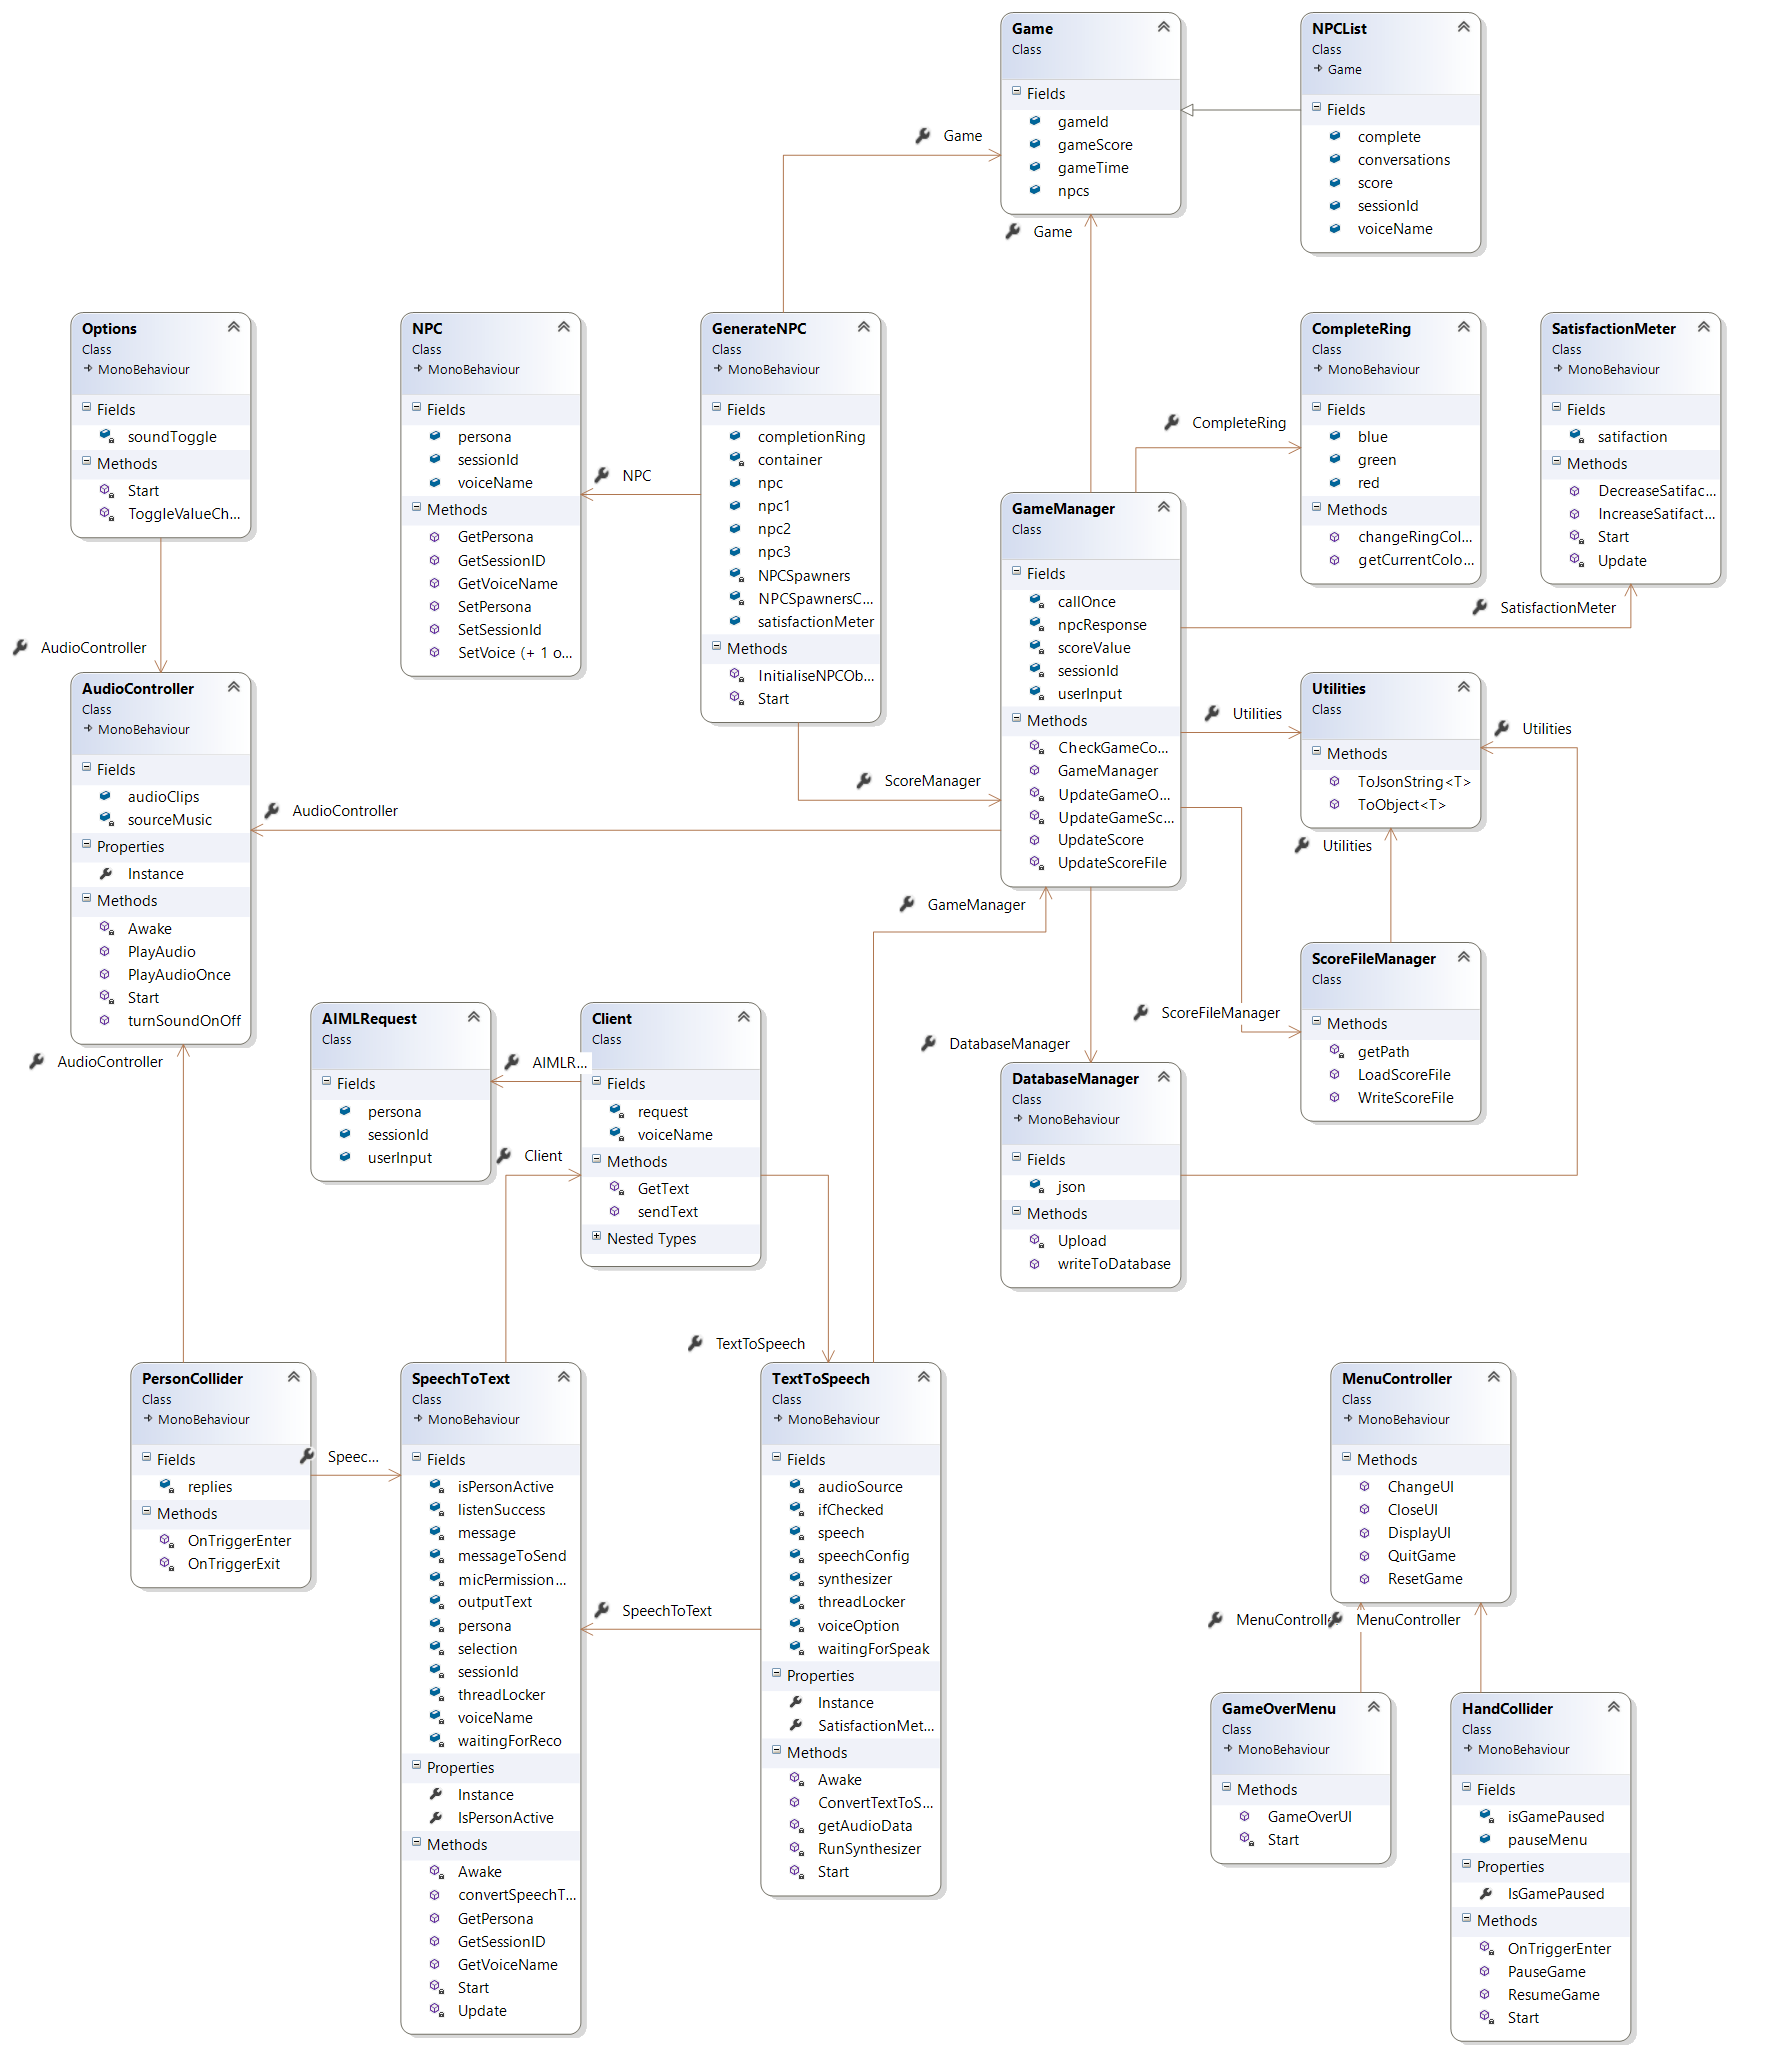
\includegraphics[width=1\textwidth]{Images/ClassDiagram.png}
\end{figure}

\subsection{3D Models}
Generating realistic bots with realistic models was a problem that was easily solved with the aid of a website called Mixamo\cite{Mixamo31:online}. This website has an plethora of high quality 3d character models along with animations. Once the model was imported into Unity all that was left to do was give these bots a session ID,whether they had a ticket or not, a random voice, a gender based on that voice and a random persona E.g. Polite, neutral and rude. These personas would aid us later in deciding which AIML file to use server-side. As seen in the below code snippet this is how we generate all these traits. The session ID is a random number between 1 and 10000. The persona is an integer between zero and three, each number meaning a different persona: 

\begin{table}[!ht]
    \centering
    
    \caption{NPC Personas \newline}
    \label{tab:my_label}
\begin{tabular}{ |p{3cm}|p{5cm}|  }
\hline
\multicolumn{2}{|c|}{NPC Personas} \\
\hline
Number & Persona \\
\hline
0 & Rude NPC \\
\hline
1 & Neutral NPC \\
\hline
2 & Polite NPC \\
\hline
\end{tabular}

\end{table}
\newpage

\begin{lstlisting}[caption={Random NPC persona generation.},label={lst:npcs}, language=python]
    public void SetSessionId()
    {
        sessionId = UnityEngine.Random.Range(1, 10000);
    }
    public void SetPersona()
    {
        persona = UnityEngine.Random.Range(0, 3);
    }
    public void SetVoice()
    {
        //0 = male 1= female
        int gender = UnityEngine.Random.Range(0, 2);
        
        string[] voicesMale = {"en-US-GuyNeural", "en-IE-Sean"};
        string[] voicesFemale = { "en-US-JessaNeural", "de-DE-KatjaNeural" };
        if (gender == 0)
        {
            int rand = UnityEngine.Random.Range(0, voicesMale.Length);
            voiceName = voicesMale[rand];
        }
        else if(gender == 1)
        {
            int rand = UnityEngine.Random.Range(0, voicesFemale.Length);
            voiceName = voicesFemale[rand];
        }
    }
\end{lstlisting}

\medskip
Once these traits have been generated all that is left to be done is to instantiate them in the virtual 3D environment. The solution to this can be seen in the below snippet. A random NPC model is chosen and oriented correctly in the environment.
This snippet is also wrapped in a for loop to generate multiple random NPCs. There is an array of manually place GameObjects in the virtual world. These GameObjects act as spawning points for a single NPC. Based on the NPCs voice a Male or Female model is loaded then it is spawned in the position and rotation of one of the spawn points according to the index of the loop. After this process is complete, we see NPCs standing in all the spawn points. This is how all the NPCs/Bots are spawned in the application.\newline
\newpage
\begin{lstlisting}[caption={NPC generation.},label={lst:npcs1}, language=python]
    if (copy.GetComponent<NPC>().GetVoiceName() == "en-US-JessaNeural" || copy.GetComponent<NPC>().GetVoiceName() == "de-DE-KatjaNeural")
    {
        int rand = UnityEngine.Random.Range(0, 2);

        // Instantiate random woman model
        if(rand == 0)
        {
            copy = Instantiate(npc2, new Vector3(NPCSpawners[i].position.x, NPCSpawners[i].position.y, NPCSpawners[i].position.z), Quaternion.Euler(0, NPCSpawners[i].rotation.eulerAngles.y, 0));
            copy.GetComponent<NPC>().SetVoice(npcVoice);
            copy.transform.parent = container.transform;
        }
        else if(rand == 1)
        {
            copy = Instantiate(npc3, new Vector3(NPCSpawners[i].position.x, NPCSpawners[i].position.y, NPCSpawners[i].position.z), Quaternion.Euler(0, NPCSpawners[i].rotation.eulerAngles.y, 0));
            copy.GetComponent<NPC>().SetVoice(npcVoice);
            copy.transform.parent = container.transform;
        }
    }
    else
    {
        // Instantiate male model
        copy = Instantiate(npc1, new Vector3(NPCSpawners[i].position.x, NPCSpawners[i].position.y, NPCSpawners[i].position.z), Quaternion.Euler(0, NPCSpawners[i].rotation.eulerAngles.y, 0));
        
        // Set the voice and add to container object.
        copy.GetComponent<NPC>().SetVoice(npcVoice);
        copy.transform.parent = container.transform;
    }
\end{lstlisting}

\medskip
Due to us not being trained in 3D modeling and animation here are some links to the models we used and altered for this project:

\begin{itemize}
    \item Train Station Model: https://assetstore.unity.com/packages/3d/environments/industrial/train-stations-bundle-161989
    \item City Chunk Model: https://assetstore.unity.com/packages/3d/environments/urban/simple-city-pack-plain-100348
\end{itemize}

\subsection{Animation}
Animations in our opinion were important in this application. We needed the user to feel as if they were speaking to a person. If the NPCs where static it would have ruined the realism, completely disconnecting the user from this virtual world. As mentioned earlier, we were fortunate to find a website called Mixamo\cite{Mixamo31:online}. As well as realistic models it also had animations to go alongside them. The process of applying the animation to the model is simple but tedious. Firstly, you must add an Animator component to the model/NPC this allows you to manage your animation clips. Once this is done, animations can be added to the animator using a graph-like interface as seen in figure~\ref{fig:anim}. Each animation is considered as a state. If certain parameters are met you can change the state, therefore changing the animation.

\begin{figure}[!ht]
    \centering
    \caption{Animator}
    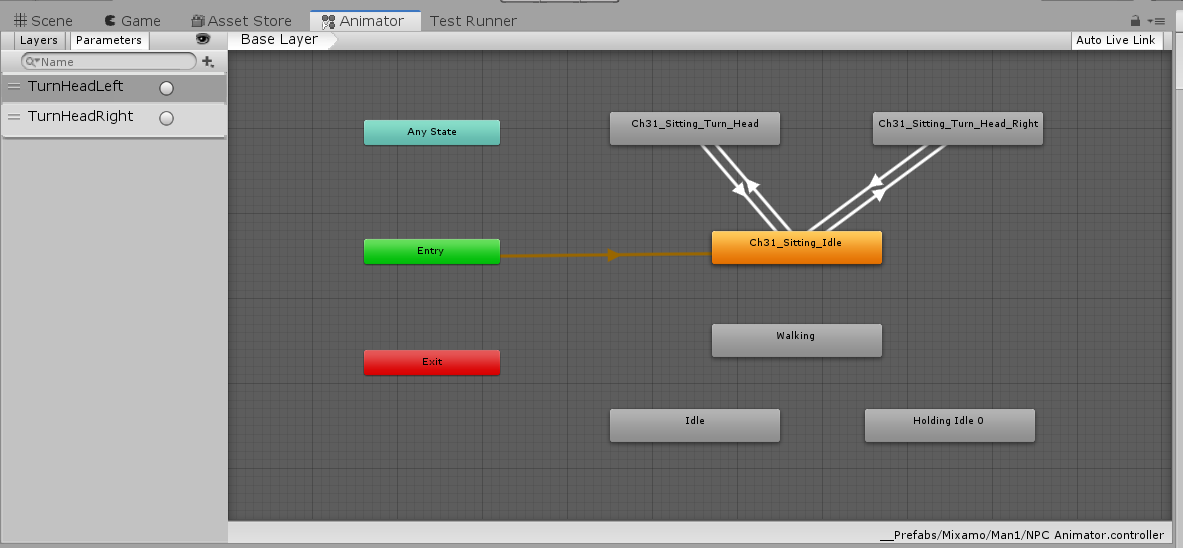
\includegraphics[width=1\textwidth]{Images/animator.PNG}
    \label{fig:anim}
\end{figure}

\newpage
\subsection{Usability/User Experience}
Throughout the development of this project we focused a lot of effort on ensuring the training application was intuitive to the user. We looked a number of areas in regards to user experience and usability which we will look at below.

\subsubsection{Passenger (NPC) Interaction}
From our initial meetings with our supervisor and the initial scope we laid out we felt getting the interaction to feel as real and immersive as possible was important. In real life, a ticket inspector can walk up to passenger and start a conversation simply by saying "Hello". We wanted our training experience to reflect this simple nature. There were a number of interaction in our development process such as initially having the player press a button to start speaking with an NPC, but we felt it was quite cumbersome and took away from the experience especially in VR. Through user testing we developed a simple way of interacting with an NPC. It involved adding a collider to each NPC which would act as a barrier. Once this barrier was passed, E.g the player moves close to the NPC it would trigger a conversation and the Azure Speech to Text service would start listening for input. Another aspect we looked at was keeping the flow of conversation intuitive. Similar to the initial interaction we felt that pressing a button wasn't suitable, so again we developed an automatic system. Once the result is returned from the Text to Speech and spoken by the passenger, the STT service will automatically start listening again for the player to reply to the passenger. For example if the player asked to see the passengers ticket, and the NPC replied with "I don't have a ticket", then the service will start listing for possible reply like "Why don't you have a ticket?". This simple flow of interaction and conversations improved the user experience drastically. More information on STT and TTS technologies can be found below in their respective sections. 

\subsubsection{Player Input}
Again from our meetings another area to improve immersion was to allow the player to psychically speak to a passenger. Our initial tests involved a keyboard input however it was very slow and cumbersome to type out each reply. We also looked at a multiple choice decisions where the player could reply with three options, however from initial user tests it was compared to a role playing decision based game rather than a immersive training experience. Instead we developed a Speech service that would listen for your voice, parse it to text to send to our chatbot for a reply. Of course this was more of a challenge as the player could say anything and in any way, however it is something that was very successful in our final build and really improved the overall experience.

\subsubsection{Passenger Information and Scoring}
There were a number of things that we wanted to display to the player about each passenger they interact with. Firstly, whether the passengers ticket had been checked on not. We decided this should be simple and researched multiple methods such as displaying a green tick beside their head and outputting a completion sound to the user amongst others. We decided that a ring around the passengers feet that would initially be red and then turn to green would work best. The ring turns to green when the player has checked the passengers ticket or dealt with situation where they don't have a ticket. It also turns blue when the player is within the range to start a conversation. This can be seen in figure~\ref{fig:interaction1}. This red, blue, green loop is very simple to grasp and worked well in the various user tests. Also it worked well for the VR experience as it is very subtle but effective in displaying the required information.

\begin{figure}[!ht]
    \centering
    \caption{Interaction with passenger.}
    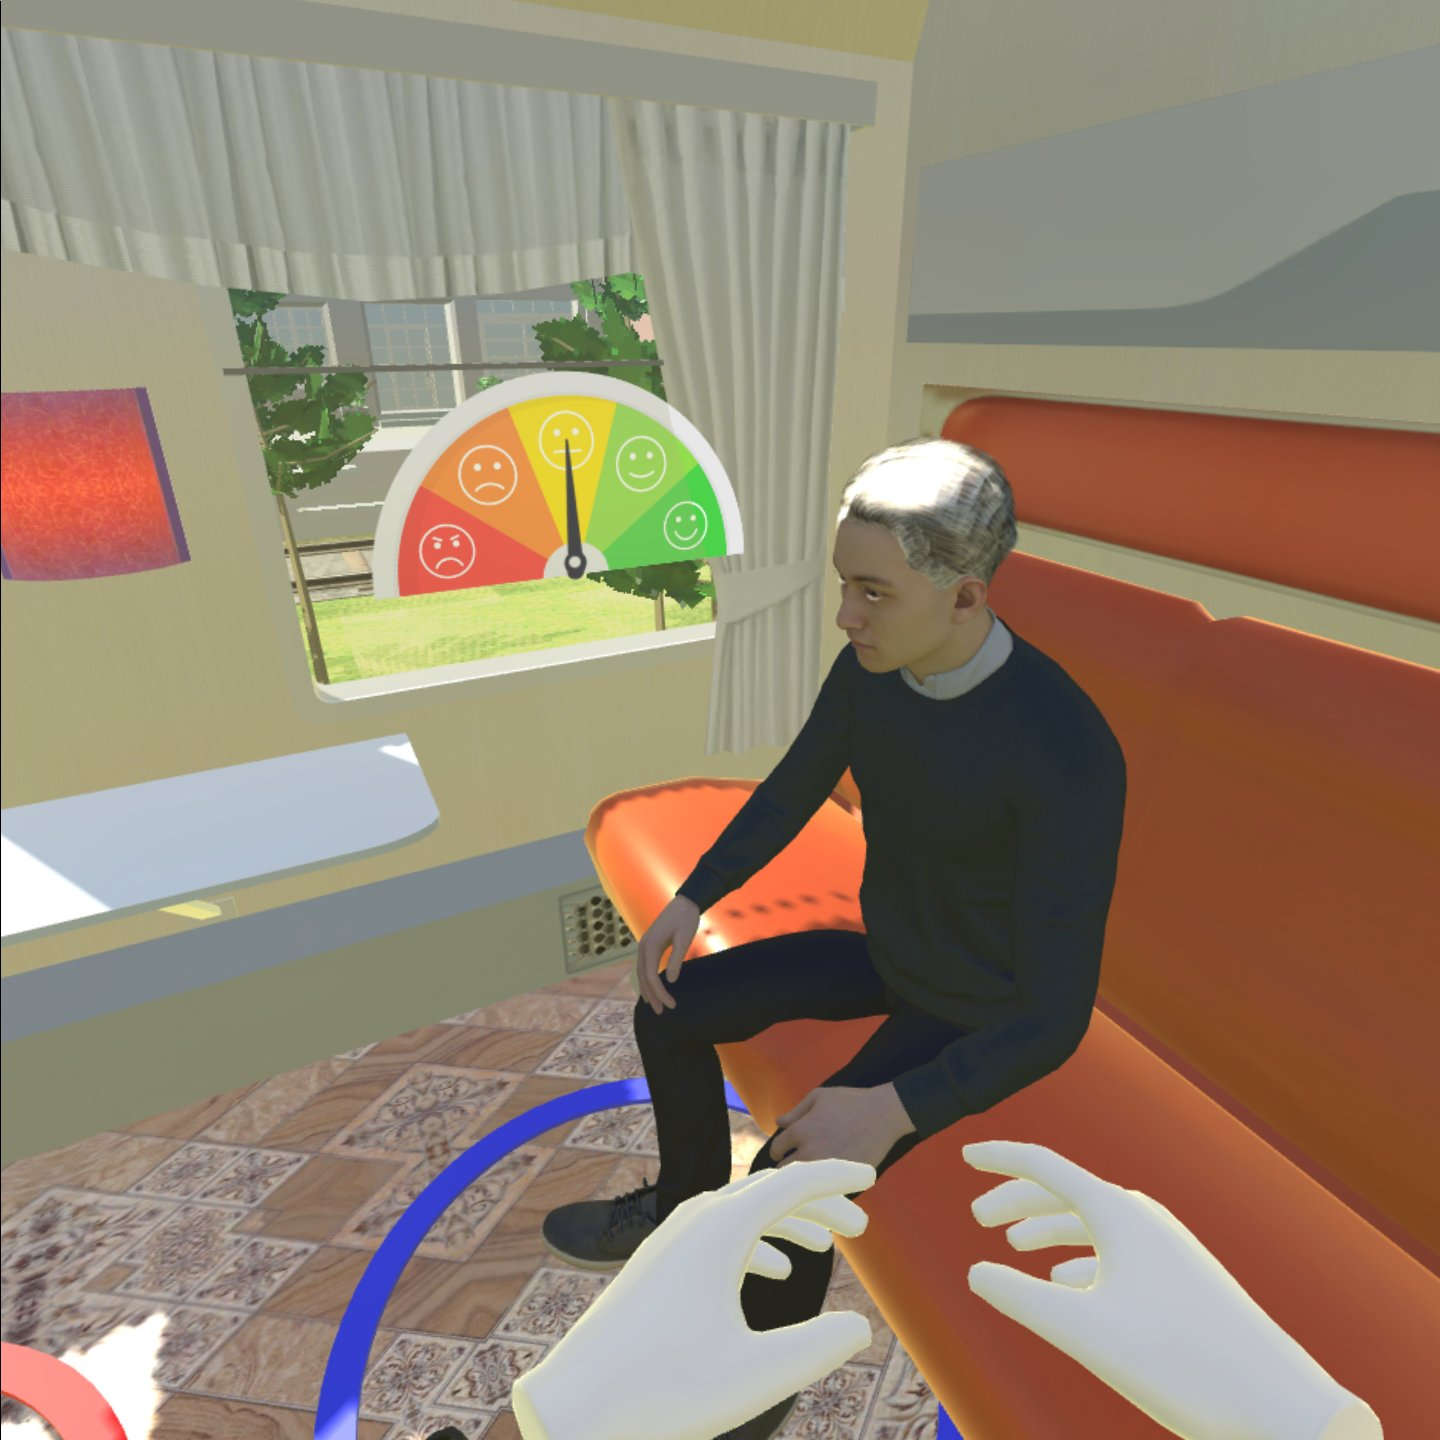
\includegraphics[width=0.8\textwidth]{Images/Interaction.jpg}
    \label{fig:interaction1}
\end{figure}

\newpage

\subsubsection{VR Support}
As our main platform focus was VR support on the Oculus Quest we wanted to ensure it was the most immersive experience possible. This was taken into account when designing the various environments (The train, the station, city etc), the in game sound, the player interactions, and controls. The controls were designed to require the least requirement of buttons possible, so the user didn't feel like they were holding controllers. All menu interactions are done by looking around in the virtual space and pulling the triggers, which is a simple fluid movement. One area we felt really improves the experience was the inclusion of the in-game watch. It was a very simple thing but it really was success in our user tests. In the virtual space we wanted to feel like the user is really in the train station to the best of our ability, and if they look down at anytime they can view their hands in real time and move their fingers. On the left hand there is a simple dialog watch that displays the real world time. If the user touches this watch with their right hand the game is paused and a virtual menu is displayed. Unfortunately, this was only a feature that could work on the VR build, but we implemented the pause menu support by displaying the menu on front of the player when the pause button is pressed.

\subsubsection{User Interface (UI) Design}
For this project we used a simple design scheme for all menus and UI. It involved a simple grey background, strong contrasting text and blue buttons. This made it easy to read and view all elements throughout the application. All menus were also designed with ergonomics in mind, so that it would be easy for the user to move between menus, close the menus or select options. For example on the pause menu implemented in VR the QUIT and RESET button were placed at the top as from testing they could be accidentally pressed when touching the watch. This can be seen in figure~\ref{image:PauseMenu} The game time is also placed accordingly along with the option to turn he sound on and off. We wanted to ensure everything required by the player is all in one place and easily accessible. This idea was reflected in the start menu and game over menu too. Figure~\ref{image:Menus} shows the layout of classes developed to handle all UI.

\begin{figure}[h!]
	\caption{UI displayed on watch.}
	\label{image:PauseMenu}
	\centering
	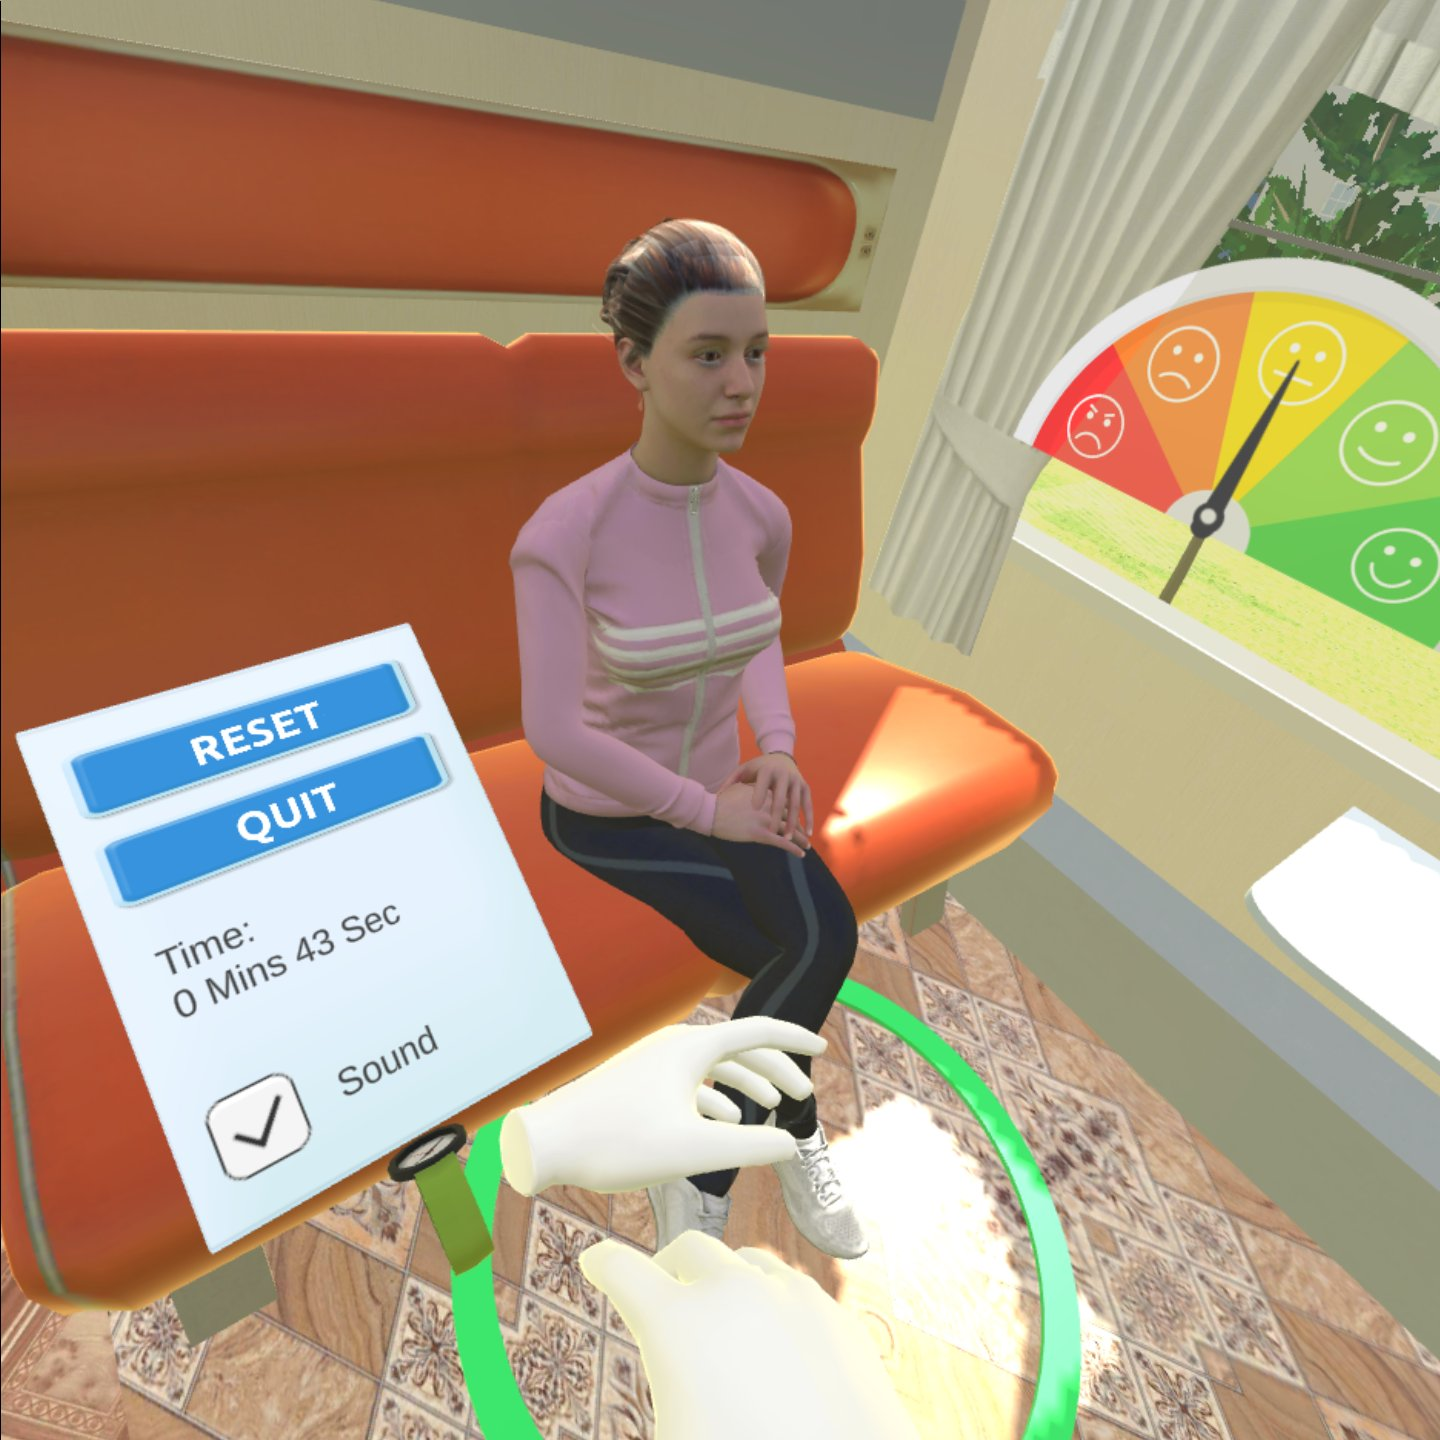
\includegraphics[width=0.8\textwidth]{Images/Interaction2.jpg}
\end{figure}

\begin{figure}[h!]
	\caption{Class Diagram - Menus}
	\label{image:Menus}
	\centering
	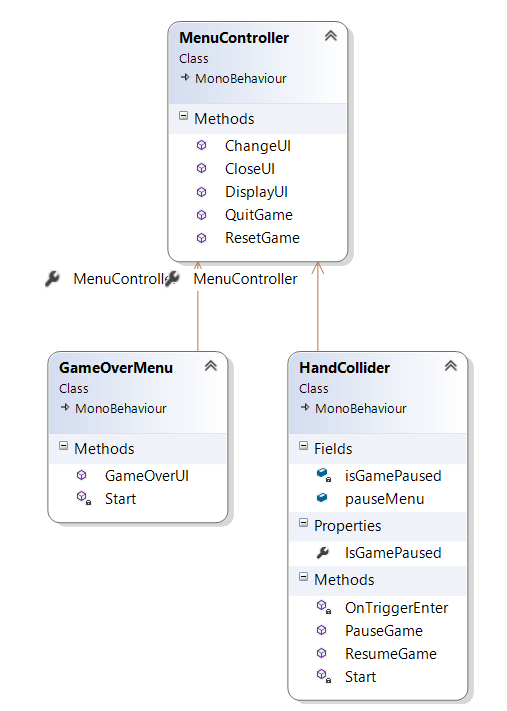
\includegraphics[width=0.6\textwidth]{Images/ClassDiagram Menus.png}
\end{figure}

\newpage

\subsubsection{Tutorial}
For this application we have also designed a tutorial scene. This scene is simply used for the trainee to learn more about the application and how it works before they get into the training environment. We used this scene to display our presentation in the project demo video required. We have also developed simple to use tutorial UI, which allows the user to scroll between pages and close when ready. An example of this can be seen in figure~\ref{image:tutorial}.

\begin{figure}[h!]
	\caption{UI Tutorial.}
	\label{image:tutorial}
	\centering
	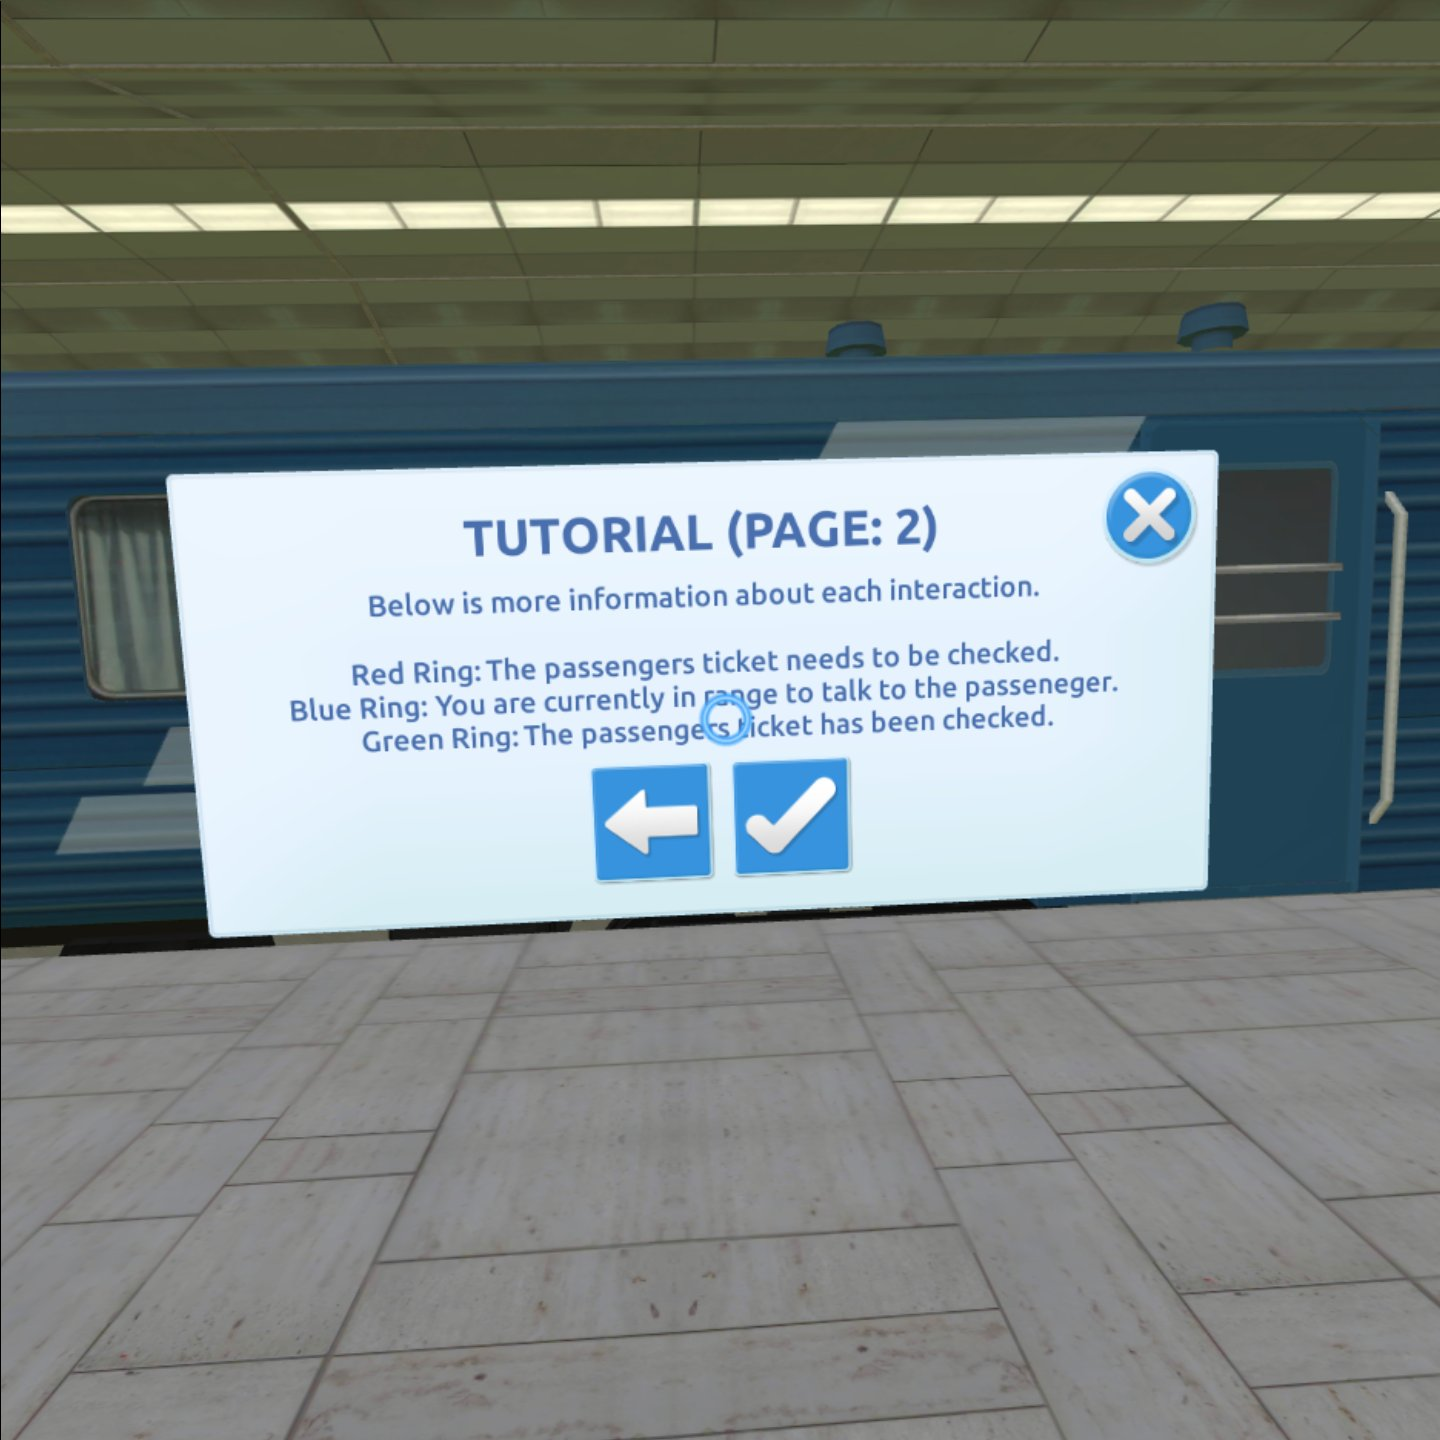
\includegraphics[width=0.6\textwidth]{Images/Tutorial.jpg}
\end{figure}

\newpage

\subsection{Scoring System}
As one of the main goals of this project was to create a useful training experience to train ticket inspectors in relation to conflict resolution, we decided it would need a scoring system to help both the trainee and the training centre. A simple system was devised for each interaction and was scored depending on user input and the way it's said. Table ~\ref{tab:scores} shows example of how the result is scored, based on the user input. If the user is deemed aggressive then they will get a -1 score, if they are deemed neutral their score won't change and if they are deemed positive they will gain one point to their total score. This simple system proved beneficial in early tests, so we implemented same idea with the personalities of each NPC.

\begin{table}[!ht]
    \centering
    
    \caption{Scores}
    \label{tab:scores}
\begin{tabular}{ |p{6cm}|p{2cm}|  }
\hline
\multicolumn{2}{|c|}{Interaction Scoring} \\
\hline
User Input & Score \\
\hline
Show me your ticket! & -1 \\
\hline
Can I see your ticket? & 0 \\
\hline
Can I see your ticket, please? & +1 \\
\hline

\end{tabular}
\end{table}

\newpage

The scoring systems works as follows as seen in Figure~\ref{image:Scoring}. Once the game is started and each NPC is being generated and template "Game" object is setup, this object contains a nested list "NPCList" which contains information about each NPC such as the conversations, current score, and sessionID. Once created it is written to a local file on the device, the decision to use file storage rather than have the object in memory was chosen for several reasons. Firstly, it allowed the file to be accessed at any time from any class easily, quickly and efficiently. It also would be stored if the game crashed, or if the user quit however results retrieval weren't implemented in the final build, it would be something to look at for future development.

\par
\medskip

The next steps occurs after each successful interaction with a NPC. The GameManager is called from the Client to update the game and score. The UpdateScore() method updates the score by reading in the current file, finding the NPC and updating their current score respectively. This also handles the check if the NPC is complete E.g. if their ticket has been checked. If the NPC is on the last state a boolean "complete" will be set to true which is used to check if the training experience is complete. This is written back out to a local file as a JSON string using the Utilities class methods. The Utilities methods were designed using generics so they can handle any type for usability. The end game condition is also checked here to see if the game is complete, if so, the end game menu is displayed with the players results.

\begin{figure}[h!]
	\caption{Scoring System Class Diagram.}
	\label{image:Scoring}
	\centering
	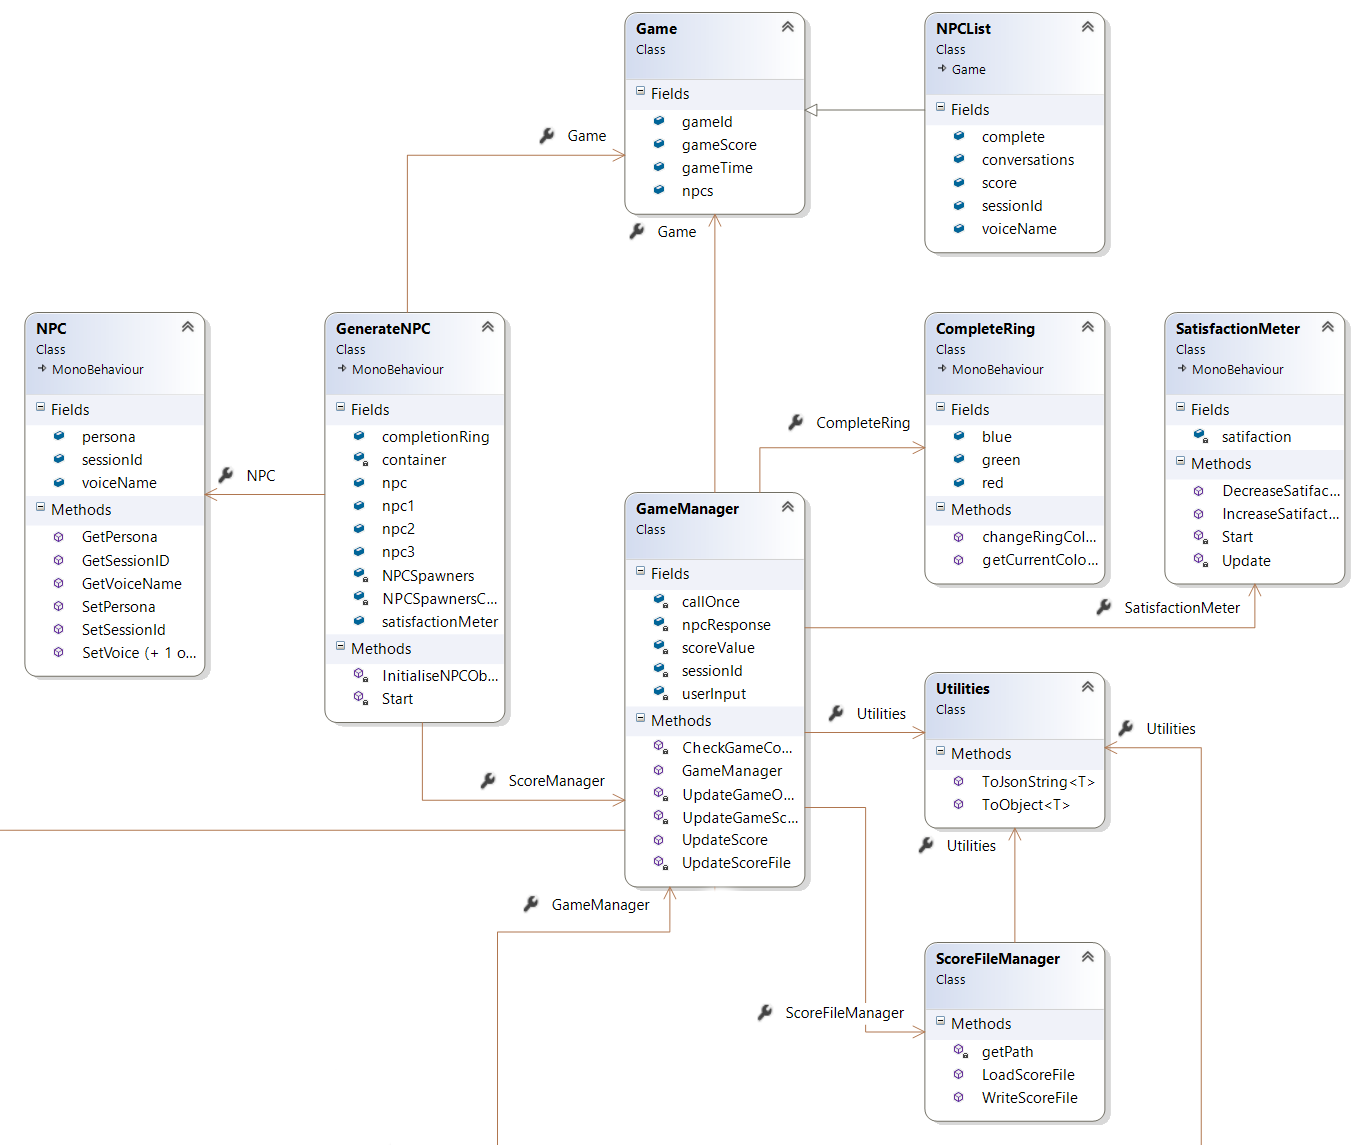
\includegraphics[width=1\textwidth]{Images/ClassDiagram Scoring.png}
\end{figure}

\newpage

\section{Azure Speech Services}
From our research and testing efforts as laid out in the technology review Azure was chosen as the provider for the speech services due to its many benefits. This provided the voice of our human like NPC's (Non-player character) and converted the players speech to machine readable diction which is sent to the Flask server for processing. Azure provides a Unity plugin to allow access to their services, with this implemented we could access the classes required.

\par
\medskip

The Speech to Text and Text to Speech functionality were the first sections to get working as it was initially decided that we would use voice commands and human speech to improve the user experience and usability rather than having the user type in their response. Using the sample Unity project provided by Microsoft as a guide we tested the implementation to learn how it works. Using this an initial prototype, the player could walk up to a cylinder which would turn blue on interaction. Once the collision occurs the speech engine begins listening and the result is returned from an Azure server as text output to the screen. We also developed a similar test build for Text to Speech where a user could input text into a text box which would play back their input as if it was spoken by a human voice. This was one of the bare essential goals of our project.

\par
\medskip

Figure~\ref{image:SpeechServices} shows the class diagram of the whole speech services in the project. The process starts in the PersonCollider class, once the player interacts with the NPC OnTriggeredEntered is fired, which sends a request to the SpeechToText class. This begins listening and displays this to the user. Once speech is recognised it is sent to Azure for processing and a result is returned as text. This is then sent to the Client which sends a HTTP request to the server as an AIMLRequest object. Once the result is processed the text is returned with a score for the chatbot to speak and the game will be updated. The TextToSpeech class handles this asynchronously and the process restarts again once the chatbot is finished talking (TTS). We will now go into more detail of how this three elements work.

\begin{figure}[h!]
	\caption{Speech Services Class Diagram.}
	\label{image:SpeechServices}
	\centering
	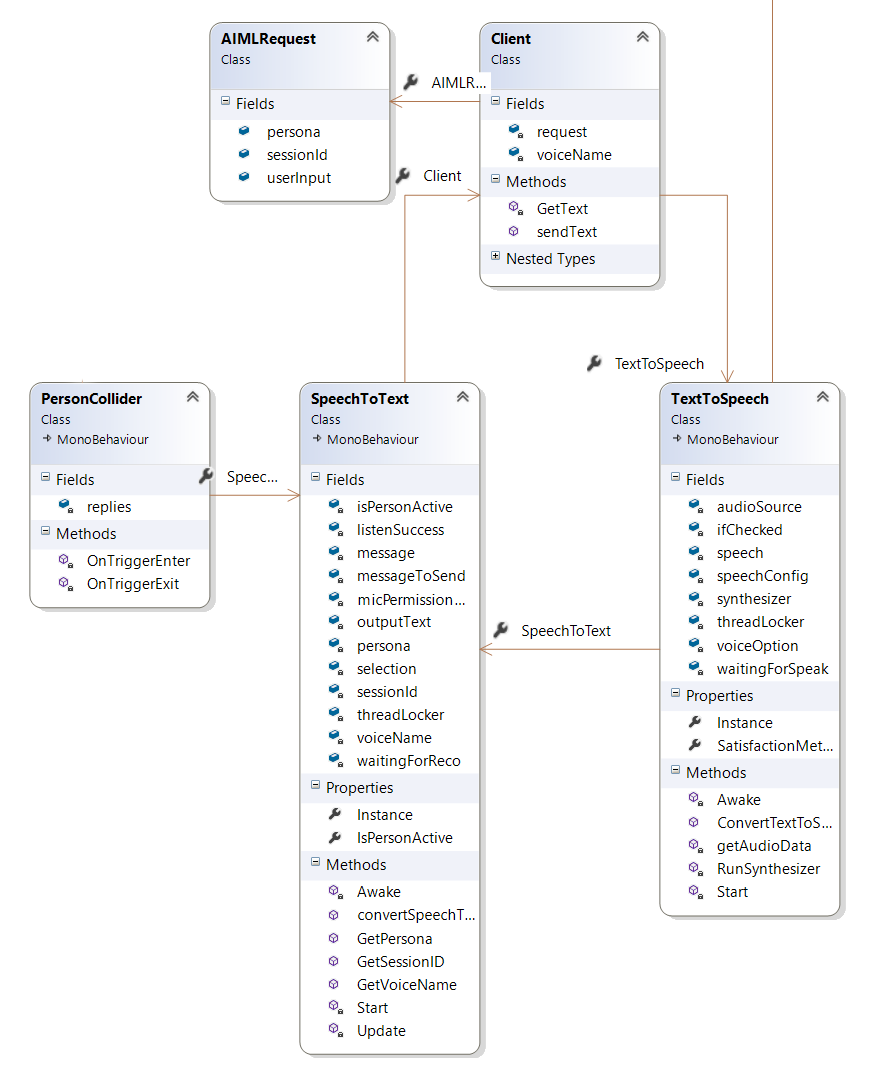
\includegraphics[width=0.8\textwidth]{Images/ClassDiagram STT and TTS.png}
\end{figure}

\subsection{Speech-to-Text}
Once this class is called a connection to the Azure services is made, then with a using statement to cut down memory usage the configuration information is passed into the imported classes (SpeechRecognizer). This begins listening for a total of 15 seconds in which it will timeout and display an error to the user. If the speech recognition is successful, the message is saved and will be sent to the client on the next update. This can be seen in Listing~\ref{lst:STT}.

\par
\medskip

Throughout the duration of the project the SpeechToText code was modified heavily to improve it in many ways, which is described below.

\begin{itemize}
  \item We had to implement a web client so it could contact the server via HTTP. More information can be found in the HTTP section in regard to the web client. We ran into problems trying to call the web client on result returned (Line 24 in Listing~\ref{lst:STT}) so instead a check was added to the Update method which checks if there is a message to be sent on each frame. If so then the returned result is sent to the server for processing.
  \item We also worked on making this Speech To Text class threaded so it would let the application continue to play when waiting for a result, as seen on line 10-13 in Listing~\ref{lst:STT}.
  \item Security was implemented by protecting the key from external access, so it is local to the device.
  \item Singleton design pattern was used as there should only be one instance of SpeechToText and it allows easy access from other classes.
\end{itemize}

\newpage
\begin{lstlisting}[caption={Speech To Text - Setup and request},label={lst:STT},language=python]
// Creates an instance of a speech config with specified subscription key and service region.
// API_Key for security this is read in from a text file and is not included on Github. 
var config = SpeechConfig.FromSubscription(API_Key, "westeurope");

using (var recognizer = new SpeechRecognizer(config))
{
    listenSuccess = false;
    messageToSend = "";

    lock (threadLocker)
    {
        waitingForReco = true;
    }

    // Starts speech recognition and returns after a single utterance is recognized. The end of a
    // single utterance is determined by listening for silence at the end or until a maximum of 15
    // seconds of audio is processed.  The task returns the recognition text as result.
    var result = await recognizer.RecognizeOnceAsync().ConfigureAwait(false);

    // Checks result.
    string newMessage = string.Empty;
    if (result.Reason == ResultReason.RecognizedSpeech)
    {
        newMessage = result.Text;

        // Set independant variables for sending the message to the server.
        listenSuccess = true;
        messageToSend = newMessage;
    }
    else if (result.Reason == ResultReason.NoMatch)
    {
        newMessage = "NOMATCH: Speech could not be recognized.";
    }
    else if (result.Reason == ResultReason.Canceled)
    {
        var cancellation = CancellationDetails.FromResult(result);
        newMessage = $"CANCELED: Reason={cancellation.Reason} ErrorDetails={cancellation.ErrorDetails}";
    }

    lock (threadLocker)
    {
        message = newMessage;
        waitingForReco = false;

        // Dispose of recognizer correctly.
        recognizer.Dispose();
    }
}
\end{lstlisting}

\subsection{Text-to-Speech}
Once this class is called a connection to the Azure services is made using the configuration information. This includes data such as the voice name which is passed from the Client. There are several voices available both male and female for different countries in the world to give a more realistic and unique experience. We choose two male and female voices from the list of Neural voices which are created using machine learning, from testing they provided the most realistic sounding voice. This can be seen in Listing~\ref{lst:TTS1}. Once setup the text is passed into the synthesizer.SpeakTextAsync() function. This is implemented using a task (Task<SpeechSynthesisResult>) so it doesn't block and wait for a response.

\begin{lstlisting}[caption={Text to Speech - Setup and request},label={lst:TTS1},language=python]
public void ConvertTextToSpeech(string inputText, string voiceName, bool ifChecked)
{
    this.ifChecked = ifChecked;

    // For security this is read in from a text file and is not included on Github. 
    string API_Key = System.IO.File.ReadAllText("../../API_Key.txt");

    speechConfig = SpeechConfig.FromSubscription(API_Key, "westeurope");
    
    // The default format is Riff16Khz16BitMonoPcm.
    // We are playing the audio in memory as audio clip, which does not require riff header.
    // So we need to set the format to Raw16Khz16BitMonoPcm.
    speechConfig.SetSpeechSynthesisOutputFormat(SpeechSynthesisOutputFormat.Raw16Khz16BitMonoPcm);

    // Change voice depending on option selected for multiple characters of different genders and ethnicities.
    speechConfig.SpeechSynthesisVoiceName = voiceName;

    lock (threadLocker)
    {
        waitingForSpeak = true;
    }

    // Creates a speech synthesizer.
    synthesizer = new SpeechSynthesizer(speechConfig, null);

    // Starts speech synthesis and returns after a single utterance is synthesized.
    // There was an issue where the game would freeze at this point "synthesizer.SpeakTextAsync(inputText)" blocks until the task is complete. 
    // To solve this, I have implemented a task which runs using a Coroutine that waits until the result from Azure is returned. 
    // Code is adapted from: https://stackoverflow.com/questions/57897464/unity-freezes-for-2-seconds-while-microsoft-azure-text-to-speech-processes-input
    Task<SpeechSynthesisResult> task = synthesizer.SpeakTextAsync(inputText);

    StartCoroutine(RunSynthesizer(task, speechConfig, synthesizer));

    lock (threadLocker)
    {
        waitingForSpeak = false;
    }
}
\end{lstlisting}

\par
\medskip

The audio response received from Azure is 16-bit mono format. The 16 bit is the bit depth, or resolution of audio. A common compact disc (CD) uses 16 bits per sample. As it's returned as bits it must be converted first to a float array to be output to the device speaker. A loop was implemented to shift the bits left on each iteration using the formula supplied in the documentation. This can be seen on line 7 in Listing~\ref{lst:TTS2}. Once completed the audio is ready for output.

\newpage
\begin{lstlisting}[caption={Text to Speech - Converting audio from bits to array},label={lst:TTS2},language=python]
private Task<float[]> getAudioData(SpeechSynthesisResult result)
    {
        var sampleCount = result.AudioData.Length / 2;
        var audioData = new float[sampleCount];

        for (var i = 0; i < sampleCount; ++i) {
            audioData[i] = (short)(result.AudioData[i * 2 + 1] << 8 | result.AudioData[i * 2]) / 32768.0F;
        }

        return Task.FromResult(audioData);
    }
}
\end{lstlisting}

\medskip
The last step of the process is to output the processed audio directly to the device speaker. A clip is first created using the data and applied to the AudioSource of the NPC and then this is played as seen in Listing~\ref{lst:TTS3}. Lastly, the SpeechToText class is called again to start the NPC listening for a new user input. However, if the NPC's ticket has already been checked this step is skipped and a predefined output is spoken, E.g "Sorry, but you have already checked my ticket.".

\begin{lstlisting}[caption={Text to Speech - Asynchronous Audio Processing},label={lst:TTS3},language=python]
private IEnumerator RunSynthesizer(Task<SpeechSynthesisResult> task, SpeechConfig config, SpeechSynthesizer synthesizer)
{
    // Wait until the task is complete E.g Azure Text to Speech returns a result.
    yield return new WaitUntil(() => task.IsCompleted);

    var result = task.Result;
    
    // Check result.
    if (result.Reason == ResultReason.SynthesizingAudioCompleted)
    {
        // Create a task to create audio data and wait till its completed.
        Task<float[]> audioTask = getAudioData(result);
        yield return new WaitUntil(() => audioTask.IsCompleted);

        // Synthesize the Audio and play to the speaker.
        // The output audio format is 16K 16bit mono
        var sampleCount = result.AudioData.Length / 2;
        var audioClip = AudioClip.Create("SynthesizedAudio", sampleCount, 1, 16000, false);
        audioClip.SetData(audioTask.Result, 0);
        audioSource.clip = audioClip;
        audioSource.Play();
        
        // true if ticket has already been checked, otherwise start listening again until ticket has been checked.
        if (!ifChecked)
        {
            // Wait until the audio is completed and start listening again.
            // Code adapted from: https://answers.unity.com/questions/1111236/wait-for-audio-to-finish-and-then-load-scene.html
            yield return new WaitWhile(() => audioSource.isPlaying);
            speech.convertSpeechToText(speech.GetSessionID(), speech.GetPersona(), speech.GetVoiceName());
        }
    }

    else if (result.Reason == ResultReason.Canceled)
    {
        var cancellation = SpeechSynthesisCancellationDetails.FromResult(result);
        Debug.Log($"CANCELED:\nReason=[{cancellation.Reason}]\nErrorDetails=[{cancellation.ErrorDetails}]");
    }

    // Dispose of synthesizer correctly.
    synthesizer.Dispose();
}
\end{lstlisting}

\par
\medskip

Throughout the project the Text To Speech code was modified and improved. Some of these improvements are outlined below.

\begin{itemize}
  \item We encountered a problem where if the the internet connection was slow the application would hang and freeze until the result was returned. From research of the documentation it was found that Microsoft developed their sample code with this problem not fixed. This problem was outlined here \cite{stackoverflow} which led it to our attention in the documentation. If "synthesizer.SpeakTextAsync()" is called it blocks and waits for a result, which was disastrous for our project as it could hang for 2/3 seconds. To fix this a asynchronous task was implemented which would allow the application to run smoothly until the audio result was played to the user. This Task<> can be seen in Listing~\ref{lst:TTS2}.
  \item Singleton design pattern was used as there should only be one instance of TextToSpeech and it allows easy access from other classes.
  \item Security was implemented by protecting the API key from external access, so it is local to the device.
\end{itemize}

\subsection{HTTP Web Client}
In order to communicate with our Flask server, we used HTTP. We did so by using the UnityEngine.Networking library. Before sending the data, we created an object to store the session ID, persona and the user input from the STT service. Once this object was created it was converted to a JSON string. Then this string of json was sent, as seen in the code snippet below, to the Flask server hosted on PythonAnywhere to be processed and return a predicted response from the bot. That response is then sent to the TTS service.

\newpage
\begin{lstlisting}[language=python]
        string json = new Utilities().ToJsonString(request);
        UnityWebRequest www = UnityWebRequest.Put("http://aaronchannon1.pythonanywhere.com/request", json);
        www.SetRequestHeader("Content-Type", "application/json");
        yield return www.SendWebRequest();

        if (www.isNetworkError || www.isHttpError)
        {
            Debug.Log(www.error);
        }
        else
        {
            string reponse = www.downloadHandler.text;

            try
            {
                string[] reponses = reponse.Split('=');

                TextToSpeech.Instance.ConvertTextToSpeech(reponses[0], voiceName, false);

                new ScoreManager(request.sessionId, Int32.Parse(reponses[1]), request.userInput, reponses[0]).UpdateScore();
            }
            catch
            { 
                TextToSpeech.Instance.ConvertTextToSpeech(reponse, voiceName, false);
            }
        }
\end{lstlisting}

\section{Chatbot - AIML}
As mentioned in the technical review, we decided to use AIML instead of a keras neural network. In listing~\ref{lst:flaskaiml} we can see the Flask GET request that also contains the AIML kernel. The kernel object controls the entire AIML library. Once the request data has been parsed, the kernel decides what aiml file to load based on their persona and if the have a ticket or not.

\begin{lstlisting}[caption={Generate AIML response},label={lst:flaskaiml},language=python]
@app.route('/request', methods=['PUT'])
def predictResponse():
     # Get json from request.
    sessionId = request.get_json()['sessionId']
    persona = request.get_json()['persona']
    userInput = request.get_json()['userInput']
    hasTicket = request.get_json()['hasTicket']

    # Load specific aiml file depending on persona and if they have a ticket.
    if hasTicket == True:
        kernel.respond("load aiml " + str(persona))
    else:
        kernel.respond("load aiml " + str(persona)+ " NO TICKET")
        
    print("DATA: ", kernel.getPredicate("usersName", sessionId))

    result = re.sub(r'([^\s\w]|_)+', '', userInput)

    # Predict reponse for specific session using user input.
    response = kernel.respond(result, sessionId)

    return response
\end{lstlisting}

Once loaded, any illegal characters are removed from the users input, making it easier to pass it into the AIML kernel. That edited input is then passed into the .respond method to get a response. From listing~\ref{lst:aiml1} we can see a stripped down version of the conversation you can have with a RUDE bot with NO ticket. As mentioned, this aiml file is loaded from the request data. The user can initiate the conversation by saying "Ticket Please". The bot then looks for a category that contains the phrase. In the case that the phrase does not exist in the AIML we have added a catch all that can be seen at the bottom of the file to generate a response if the bot does not understand what you are trying to say. In the case of saying "Ticket please", once found, the bot has a few random options it can response with. These options can be seen under the random tag. The bot clearly doe not want to talk to you right now. You can continue by saying " I'm sorry you need a ticket". Even though this phrase is not directly in the list of categories however, a form of it is: "$<$pattern$>$* YOU NEED A TICKET$</$pattern$>$". The star symbol(*) allows you to say any number of words before "YOU NEED A TICKET" making it AIML great in catching most scenarios. The bot says that it does not have a ticket. The next part is up to the user. Do they let them away with not having a ticket or tell them that they have to pay a fine? If the user tells them to "BRING ONE NEXT TIME" the rude bot will reply with "Yeah I will. Can you leave me alone now?=3". The "=3" at the end of the reply indicates to us on the Unity client side that the conversation with that bot is now complete and deactivates them. In the case that you ask them to pay the fine, they respond rudely and you must tell then to calm down. After this the bot can decide whether they'd rather pay the fine or make sure to bring one next time.

\begin{lstlisting}[caption={Generate AIML response},label={lst:aiml1},language=XML]
    <category>
      <pattern>TICKET PLEASE</pattern>
      <template>
         <random>
            <li> I'm busy.</li>
            <li> Can't you see I'm busy</li>
            <li> I don't have time for this!</li>
         </random>
      </template>
   </category>
   
    <category>
      <pattern>* YOU NEED A TICKET</pattern>
      <template>
        <random>
            <li> Well I don't have one</li>
            <li> Go away, I don't have one</li>
            <li> Stop bothering me I don't have one!</li>
         </random>
      </template>
   </category>
   
    <category>
      <pattern>BRING ONE NEXT TIME</pattern>
      <template>
            Yeah I will. Can you leave me alone now?=3
      </template>
    </category>
    
    <category>
      <pattern>* PAY THE FINE</pattern>
      <template>
            Piss off! I'm not paying the fine!
      </template>
    </category>

    <category>
      <pattern>* CALM DOWN</pattern>
      <template>
        <random>
            <li> Okay, I'll make sure to bring one next time=3</li>
            <li> I'd rather pay the fine=3</li>
         </random>
      </template>
    </category>
    
    <!-- CATCH ALL -->
   <category>
    <pattern>*</pattern>
        <template>
         <random>
            <li>Can you repeat that?=1</li>
            <li>What?=1</li>
            <li>I don't understand=1</li>
            <li>Pardon?=1</li>
            <li>Excuse me?=1</li>
         </random>
      </template>
    </category>
\end{lstlisting}

The listing~\ref{lst:aiml1} is a simplified version of a rude bot with no ticket. An AIML file has been constructed for each persona (polite, neutral and rude). Also, another three AIML files were created for those personas that do not have a ticket. Totaling to six AIML files which all can be found on the Github repository.


\section{Back-end - Flask}
After some consideration as described in the Technical review, we decided a Flask server would be best to handle the back-end. Firstly we set up a simple Flask server that could handle a simple GET request and return some text which can be seen in Listing~\ref{lst:flask1}. It was important to create this simple GET request for testing purposes. We could just test that we could make a HTTP request and if it returned a response, we knew the server was working correctly.\newline


\begin{lstlisting}[caption={Basic Flask GET request},label={lst:flask1},language=python]
from flask import Flask, jsonify, request, json
from flask_pymongo import PyMongo
import aiml
import os, requests, time
from xml.etree import ElementTree

@app.route('/')
def index():
    return "<h1>Welcome!!</h1>"
    
if __name__ == "__main__":
    app.run(debug=True)
\end{lstlisting}

\medskip
Once the simple Flask server was setup it was time to implement the AIML request. This request would contain data like the session ID, NPC person and the user input from the STT service. Because of this it had to be a PUT method as seen in Listing~\ref{lst:flask2}. We can also see in lines 4-6, the JSON data from the request being converted back into their respectable types. As mentioned in Section 4.4 here is where all the AIML code is located too. Once AIML has generated an output from the input this output is sent back to the Unity client to be converted back into speech using the Azure TTS service. 

\begin{lstlisting}[caption={Flask PUT request to generate AIML response.},label={lst:flask2},language=python]
@app.route('/request', methods=['PUT'])
def predictResponse():
     # Get json from request.
    sessionId = request.get_json()['sessionId']
    persona = request.get_json()['persona']
    userInput = request.get_json()['userInput']
    hasTicket = request.get_json()['hasTicket']

    # Load specific aiml file depending on persona and if they have a ticket.
    if hasTicket == True:
        kernel.respond("load aiml " + str(persona))
    else:
        kernel.respond("load aiml " + str(persona)+ " NO TICKET")
        
    print("DATA: ", kernel.getPredicate("usersName", sessionId))

    result = re.sub(r'([^\s\w]|_)+', '', userInput)

    # Predict reponse for specific session using user input.
    response = kernel.respond(result, sessionId)

    return response
\end{lstlisting}

The final part of the Flask server is another PUT request that, once the training session is finished, pushes all the session's data to a Mongo database. This can be seen in Listing~\ref{lst:flask3}. Simpler to the AIML put request, all that JSON data is converted back into types. This data includes the session/game's ID, the score of the user, the time it took and all the NPCs. Once this data has being inserted into the Mongo database a response is returned stating that the insertion was successful. 

\begin{lstlisting}[caption={Flask PUT request to Push Data to MongoDB},label={lst:flask3},language=python]
@app.route('/api/results', methods=['PUT'])
def uploadResult():
    # Get json from request.
    gameId = request.get_json()['gameId']
    gameScore = request.get_json()['gameScore']
    gameTime = request.get_json()['gameTime']
    npcs = request.get_json()['npcs']

    # Get collection from database.
    result = mongo.db.results
    
    # Write json object to MongoDB database.
    result.insert({
        'gameId': gameId,
        'gameScore': gameScore,
        'gameTime': gameTime,
        'npcs': npcs
    })

    return jsonify(data="Result sucessfully uploaded.")
\end{lstlisting}

\section{Hosting - PythonAnywhere}
After creating an account, the steps to hosting a flask server on PythonAnywhere pretty tedious. Especially if you did not create the Flask server from scratch on the site.

\begin{itemize}
    \item Firstly, you create a web app. This will generate all the necessary files you need to start.
    \item Then we added all our server files to the web app fold that was generated.
    \item Unfortunately, we had not developed the flask server on PythonAnywhere from the beginning so we had to install all the extra libraries at once before we could even get a simple get request working. To install the relevant libraries, we had to open a bash console and pip3.7 install --user "LIB-NAME" for every import we had.
    \item Then you must add every import to the WSGI config file.
\end{itemize}
After all this everything worked flawlessly, and we were able to get predictions from the Flask server.

\section{Database - MongoDB}
We have used a MongoDB database to store the final game information securely and efficiently. More information on how this is implemented can be found in the "Backend - Flask" section. We choose mLab to host this database. mLab is a fully fledged cloud provider that allows users to easily access and host their database without the need for a virtual machine. Once an account was created and the hosting service was setup using a Amazon Web Services virtual machine, the flask server could easily be connected to using credentials. These credentials are stored in an environments file and read in. This environments file is not published to our GitHub repository for security reasons. 

There were a number of issues getting MongoDB with mLab to work with our hosting service PythonAnywhere but with the correct imports and a number of tests we got it work correctly.

\subsection{Database Schema}
The database schema was designed to only include the information that would be useful to the client for training purposes. Below is a descriptions of each of the fields and why they were included. The design can be seen in listing~\ref{lst:schema}.

\begin{itemize}
  \item gameId - unique ID for each training session. This would be used to pull information about the session when required.
  \item gameScore - An overall game score to rank sessions.
  \item gameTime - The time taken by the trainee. If a trainee was rushing or took too long it could give a negative outlook.
  \item npcs - A list of all passenger interactions in one training session. Each NPC has an array index which contains information such as their session id, if there ticket was checked, their score, voice name and finally a list of the whole conversation thread with said passenger. The voice name could be used to see how a trainee would react to different genders or mixed races. The list of conversations is very useful so that the trainer can see the way the trainee deals with situation based on their reply. These fields can be seen in listing~\ref{lst:schema}. 
\end{itemize}

\newpage
\begin{lstlisting}[caption={MongoDB database schema},label={lst:schema},language=python]
    "gameId": 200,
    "gameScore": 1,
    "gameTime": "Time:\n0 Mins 20 Sec",
    "npcs": [
        {
            "sessionId": 6591,
            "complete": True,
            "score": 1,
            "voiceName": "de-DE-KatjaNeural",
            "conversations": [
                "Do you have a ticket?",
                "Here you go!"
            ]
        }
    ]
\end{lstlisting}

\subsection{Unity Connection}
How this works on the Unity side can be seen in Figure~\ref{image:Database}. It works very similar to how the client connects to the server for AIML requests and uses the same methods. A connection is made using a HTTP request that passes the data defined in listing~\ref{lst:schema} to flask server. This data is then stored using our MongoDB database hosted through mLab.

\begin{figure}[ht]
	\caption{Database Class Diagram.}
	\label{image:Database}
	\centering
	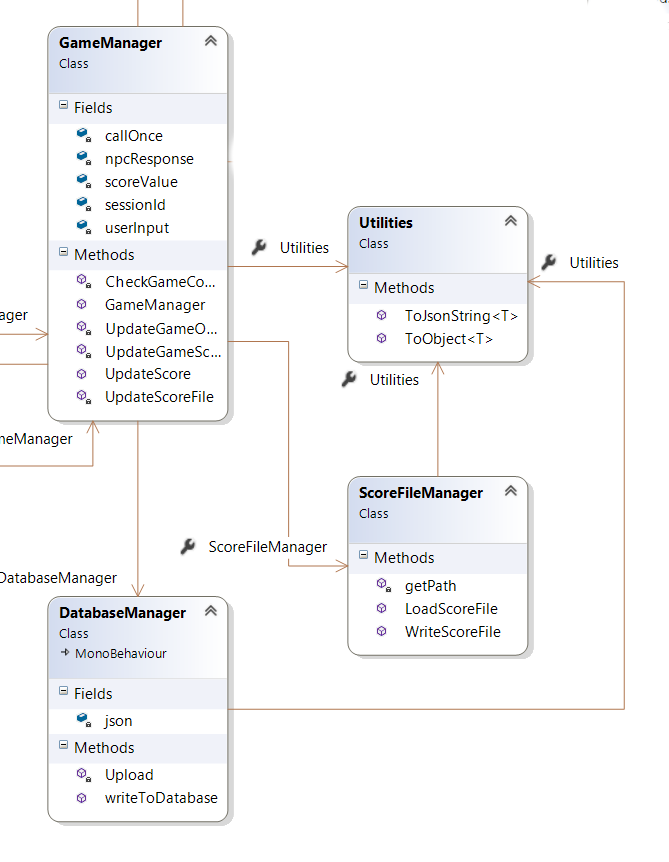
\includegraphics[width=0.8\textwidth]{Images/ClassDiagram Database.png}
\end{figure}

\newpage

\section{Code Design}
With our experience from a number of modules throughout our Software Development course, we have implemented our best knowledge in the following areas to provide a well written and efficient piece of software.

\subsection{Design Patterns and Principles}
A design pattern is blueprint used to solve common problems in software development. They are used to improve code readability and efficiency. 

\subsubsection{Singleton}
The Singleton pattern has been implemented in a number of cases that require one instance of it. For example this pattern can be seen in the AudioController script and in listing~\ref{lst:Singleton}. This would ensure there was only one instance of the class created as there should only be one audio system. It also allowed it to work easily across multiple scenes such as the tutorial and start menu.

A Singleton is created by creating a private constructor so that no other classes can create an instance of that class. The second step is to create a static instance of the class which acts as the constructor. If the instance is null then create and instance once and store it, so further calls access this cached instance. This can be seen again in listing~\ref{lst:Singleton}

\begin{lstlisting}[caption={Singleton - implemented in the AudioController script.},label={lst:Singleton},language=python]
public static AudioController Instance { get; private set; }

private void Awake()
{
    if (Instance == null)
    {
        Instance = this;
    }
}
\end{lstlisting}

\subsubsection{Single Responsibility Principle (SRP)}
SRP ensures that every class has one single purpose. E.g so there isn't classes that are handling multiple tasks. At all levels throughout the design SRP is upheld as every class has specific purpose that delegates to other classes as required.

\subsubsection{Open Close Principle (OCP)}
OCP allows classes to be open for extension but closed for modification. So multiple clients, databases, speech engines etc could be added without breaking the overall implementation.

\subsubsection{Dependency Inversion Principle}
No higher-level modules or scripts depends on a low-level module. 

\subsubsection{Law of Demeter}
No single function knows the whole navigation structure of the system. All common functionality is subjugated into multiple methods and reused where possible.

\subsection{Object Pooling}
To save on system memory in regarding the 3D objects in the Unity engine we decided to use object pooling. What this entails is loading one model into memory and it is just duplicated preventing us from having to instantiate a new model every time. An example of this in the project is the City chunk model that spawns when you are on the train. One chunk is instantiate and every other chunk is a copy of that first one. Once the copy is out of view it is then deleted, therefore saving more system memory. Another example of this can be seen in start screen with the NPC models walking in the station. There is only three models and the rest of them are copies of the initial models. This was extreme important from a system design point of view. The reason being, we were developing this application for the Oculus Quest. The Quest is currently running an old enough version of Android, Android 7.1.1 to be exact. Because the Quest is running on an mobile operating system with mobile level specifications we needed to make sure it ran smoothly and Object pooling helped us achieve this.

\subsection{Modularity}
Even though at a glance the project seems pretty glued down, meaning it is a training simulation for ticket inspectors and that it. However, the system is designed in such a way that certain components can be swapped and changed to give the user a different training experience. For example, to change the dialog of the NPCs all you have to do is simply change their AIML scripts. Now you have bots that are not just passengers on a train. To further the modularity, the entire scene can be changed in Unity with different models to give a different feel. Those are the only two things you would have to change in the entire project to create a training simulation for any other line of work.

\section{Platforms}
As we were developing for Windows, Android and VR with a focus on VR we had to ensure everything we developed would work on all platforms. This was a big challenge but we developed in such a way that all features would port across easily. However some features did have to be designed slightly different such as the watch menu implementation described above which could only be possible in VR. However, we have successfully developed a system that works correctly on all platforms.
\chapter{System Evaluation}
Blah......
\chapter{Conclusion}
This chapter provides a final outlook on the project, a summary of how we met our initial goals, the insights and knowledge we gained and some thoughts on possible future developments.

\section{Project goals}
From the initial project scope laid out in the Introduction chapter we have met these goals within the required time frame, and improved upon them in multiple ways.

\section{How we achieved our goals}
\begin{itemize}
    \item Project scope and goals were achieved and exceeded. We have built a fully fledged training application that allows a user to move around a virtual environment in VR and interact with NPC's to check their ticket. All interactions are scored and data is stored securely on a database (MongoDB). A lot of work went into improving the user experience, the look and feel of the application and usefulness of training provided to the user. 

    \item Using a Mixed Research Methodology allowed us to gain knowledge throughout the whole project. Also using Extreme Programming (XP) as our development methodology ensure code quality was upheld always, as a working build was always available for each meeting.
    
    \item We put a big emphasis on testing to utilities XP to it's full potential. With this we implemented ...
    
    \item We designed and developed the application to be fully modular so that new technologies, new scenarios, new languages and much more could be implemented with further development.

\end{itemize}


\section{Findings and Insights gained}
% based on system Evaluation

Throughout the project there were a number of trial and error issues that come with working with new technologies and hardware, but they all worked out due to our development methodologies. One example of such an error was when building to the Oculus Quest, the Azure Speech Services would stop working once the application was closed and opened again. This was a major problem as the application could only be used once. From research of possible solutions and checking the error logs output by the Oculus Quest we came to a solution which we had thought would fix it. The Quest was throwing an error in regard to a .dll file it couldn't find. A number of people had a similar issue on a forum post, and the suggestion was to change the Unity version. To test this we built a new basic version of the project in Unity 2018, however the error still persisted when everything was added in. Going through each addition it was found that the error was caused by an Avatar game object that was added to the VR camera. This Avatar game object allows the user to see their own personal avatar in game connected to an Oculus account. It is useful for multiplayer games but not required for our application, but it is a standard addition to the supplied VR camera that Oculus provides so we would have never found this error without going through all possible options. With this fixed we felt we could help someone that had a similar error due it's difficulty to fix, so we commented in the original forums as these people could have had the same issue but never known about it. Also, we made an issue on the official GitHub repository for Azure Speech Services so hopefully it could be useful to anyone using our same setup of technologies.

\section{Future development}
Throughout development we had multiple different ideas from either our own minds or through our supervisor meetings that weren't core to our initial project goals. However, they would be features we'd like to look at again if we were to develop the project further. Some of these ideas are as follows.
\begin{itemize}
    \item Implement language support for the training application. Currently the AIML chatbot can only interpret English, and response to English queries. As the training centre is based in Ireland this is what the client required. However, due to the fact Azure STT and TTS can detect and output multiple languages without intervention it would be possible to implement this feature without changing the project structure or adding many new technologies. A possible way this could be achieved is the server would convert any user input to English which would be compared with the predefined AIML diction we have developed. This conversion could be done using Google Translate API which is freely available for development.
    
    \item More scenarios could be implemented. For our final build we have developed a scene and tutorial focused on checking passengers tickets as outlined by our client. However, as we built the project in a modular way this could easily be expanded to included a new conflict resolution scenario for training security guards or other kinds of workers that deal with the general public. 
    
    \item A web application could be developed to view the results of each training session, and even compare results on a graph. This would be more suited if being used by multiple training centres and if the project was developed and sold as a product that customers could purchase. Each individual centre could create an account and display their own set of testing data, that the application provides. However for this project as we were working with a single client the application is set up to work with their business only, using a predefined ID for security purposes. However the database could easily be set up to handle multiple business ID's.
    
\end{itemize}

\section{Final thoughts}
\subsection{Matthew}
This project was extremely enjoyable to work on and will serve me well in my future career as a machine learning engineer. I got to work with various new technologies such as speech services, VR technology, cloud hosting providers (Heroku) and machine learning chatbots (Keras). I also improved my current knowledge using technologies such as Unity, Python, C\#, Flask and much more. I learned a lot in regards to working in a team, which suits my work flow very well. Working each week with our supervisor and with my project partner using Extreme Programming was useful especially for meeting our deadlines as the project was in a working state after each build. The research that was undertaken throughout the whole project was extremely interesting and it was great to get an insight into some of the exciting technologies out there today. Lastly, I am very happy with how the project turned and how we met our initial goals and exceeded them.

\subsection{Aaron}
\chapter{Appendices}

Here we will briefly describe the structure of the Github repository and how to install the project:

\section{Github Repo}
Github link: https://github.com/MatthewSloyan/final-year-applied-project-and-minor-dissertation
\begin{itemize}
    \item Chatbot: This folder contains the python flask server along with the AIML files. There is also a test Keras chatbot that was used during research.
    \item Dissertation: This folder contains all disseration material.
    \item Presentation: This folder contains the slide material along with a video presentation.
    \item Research: This folder contains all the research that was performed prier to development.
    \item UnityEngine: This folder contains the entire Unity side of the project. This includes all assets scripts etc.
\end{itemize}
\newpage
\section{How to Run}
Here we will explain how to download and install the project for the Oculus Quest:
\begin{enumerate}
    \item Download or clone the GitHub repo
    \item Add Unity 2019.2.6f1 to your Unity Hub. 
    \item Navigate to the "UnityEngine" and add the FinalYearProject folder to your Unity projects in Unity Hub.
    \item Launch the project.
    \item Once the project is open connect your Oculus Quest to your PC.
    \item Navigate to "File" then "Build Settings".
    \item Highlight Android under platforms and click "Switch Platform".
    \item With your Oculus Quest connected, click "Build and Run".
    \item The application will then be build and run on the Oculus.
\end{enumerate}

As the server is hosted on PythonAnywhere there is no need to make anymore change to connect to the server and it should connect by default.

%----------------------------------------------------------------------------------------
\bibliographystyle{unsrt}
\bibliography{references.bib}
\end{document}